\section{Methods}\label{sec:Material and methods}

\subsection{Alloy Design Methodology}

\subsubsection{Design Space Definition and Compositional Constraints}

In this work, we consider an 8-dimensional HEA system based on the elements Al, V, Cr, Mn, Fe, Co, Ni, and Cu. This material system Al-V-Cr-Mn-Fe-Co-Ni-Cu and all its potential subsystems from 5 to 8 elements, was selected based on the initially studied Al-V-Cr-Fe-Co-Ni system\cite{hastings2025acceleratedmultiobjectivealloydiscovery}, with the inclusion of Cu and Mn. The decision to include Mn and Cu in the alloy system was motivated by their distinct contributions to the mechanical and microstructural properties of high-entropy alloys (HEAs). Manganese is known to enhance ductility and toughness, while copper improves corrosion resistance. These additions expand the versatility of the alloy system, enabling a broader exploration of composition-property relationships. 

%Unlike the previous study, which imposed strict constraints on thermal and mechanical properties, 
This study is more expansive and operates under an open-ended design strategy. The only enforced constraint is phase stability, ensuring a single-phase FCC structure across the designated temperature range. This open-ended approach aims to facilitate exploration without prematurely excluding any regions of the composition space. %In this study, we moved away from the constraint satisfaction and optimization approach in the previous work, where phase stability and additional properties were used to constrain the design space. 
By maintaining a broader scope, we aim to capture a wider variety of high-performing alloys while systematically managing the complexity of the design space.

The initial compositional space is discretized at a resolution of 4 atomic percent, resulting in a pool of 3,365,848 unique compositions. To ensure manufacturability and focus on regions with potential for high performance, expert recommendations were used to impose upper limits on elemental fractions: Al $\leq 0.24$, V $\leq 0.24$, Cr $\leq 0.50$, Mn $\leq 0.40$, Fe $\leq 0.50$, Co $\leq 0.50$, Ni $\leq 0.60$, Cu $\leq 0.24$. These compositional maximums reduce the design space to 1,490,129 candidate alloys, ensuring that the search is confined to regions that are likely to yield feasible and mechanically robust materials. %recheck the wording. 

\begin{figure}[htbp]
    \centering
    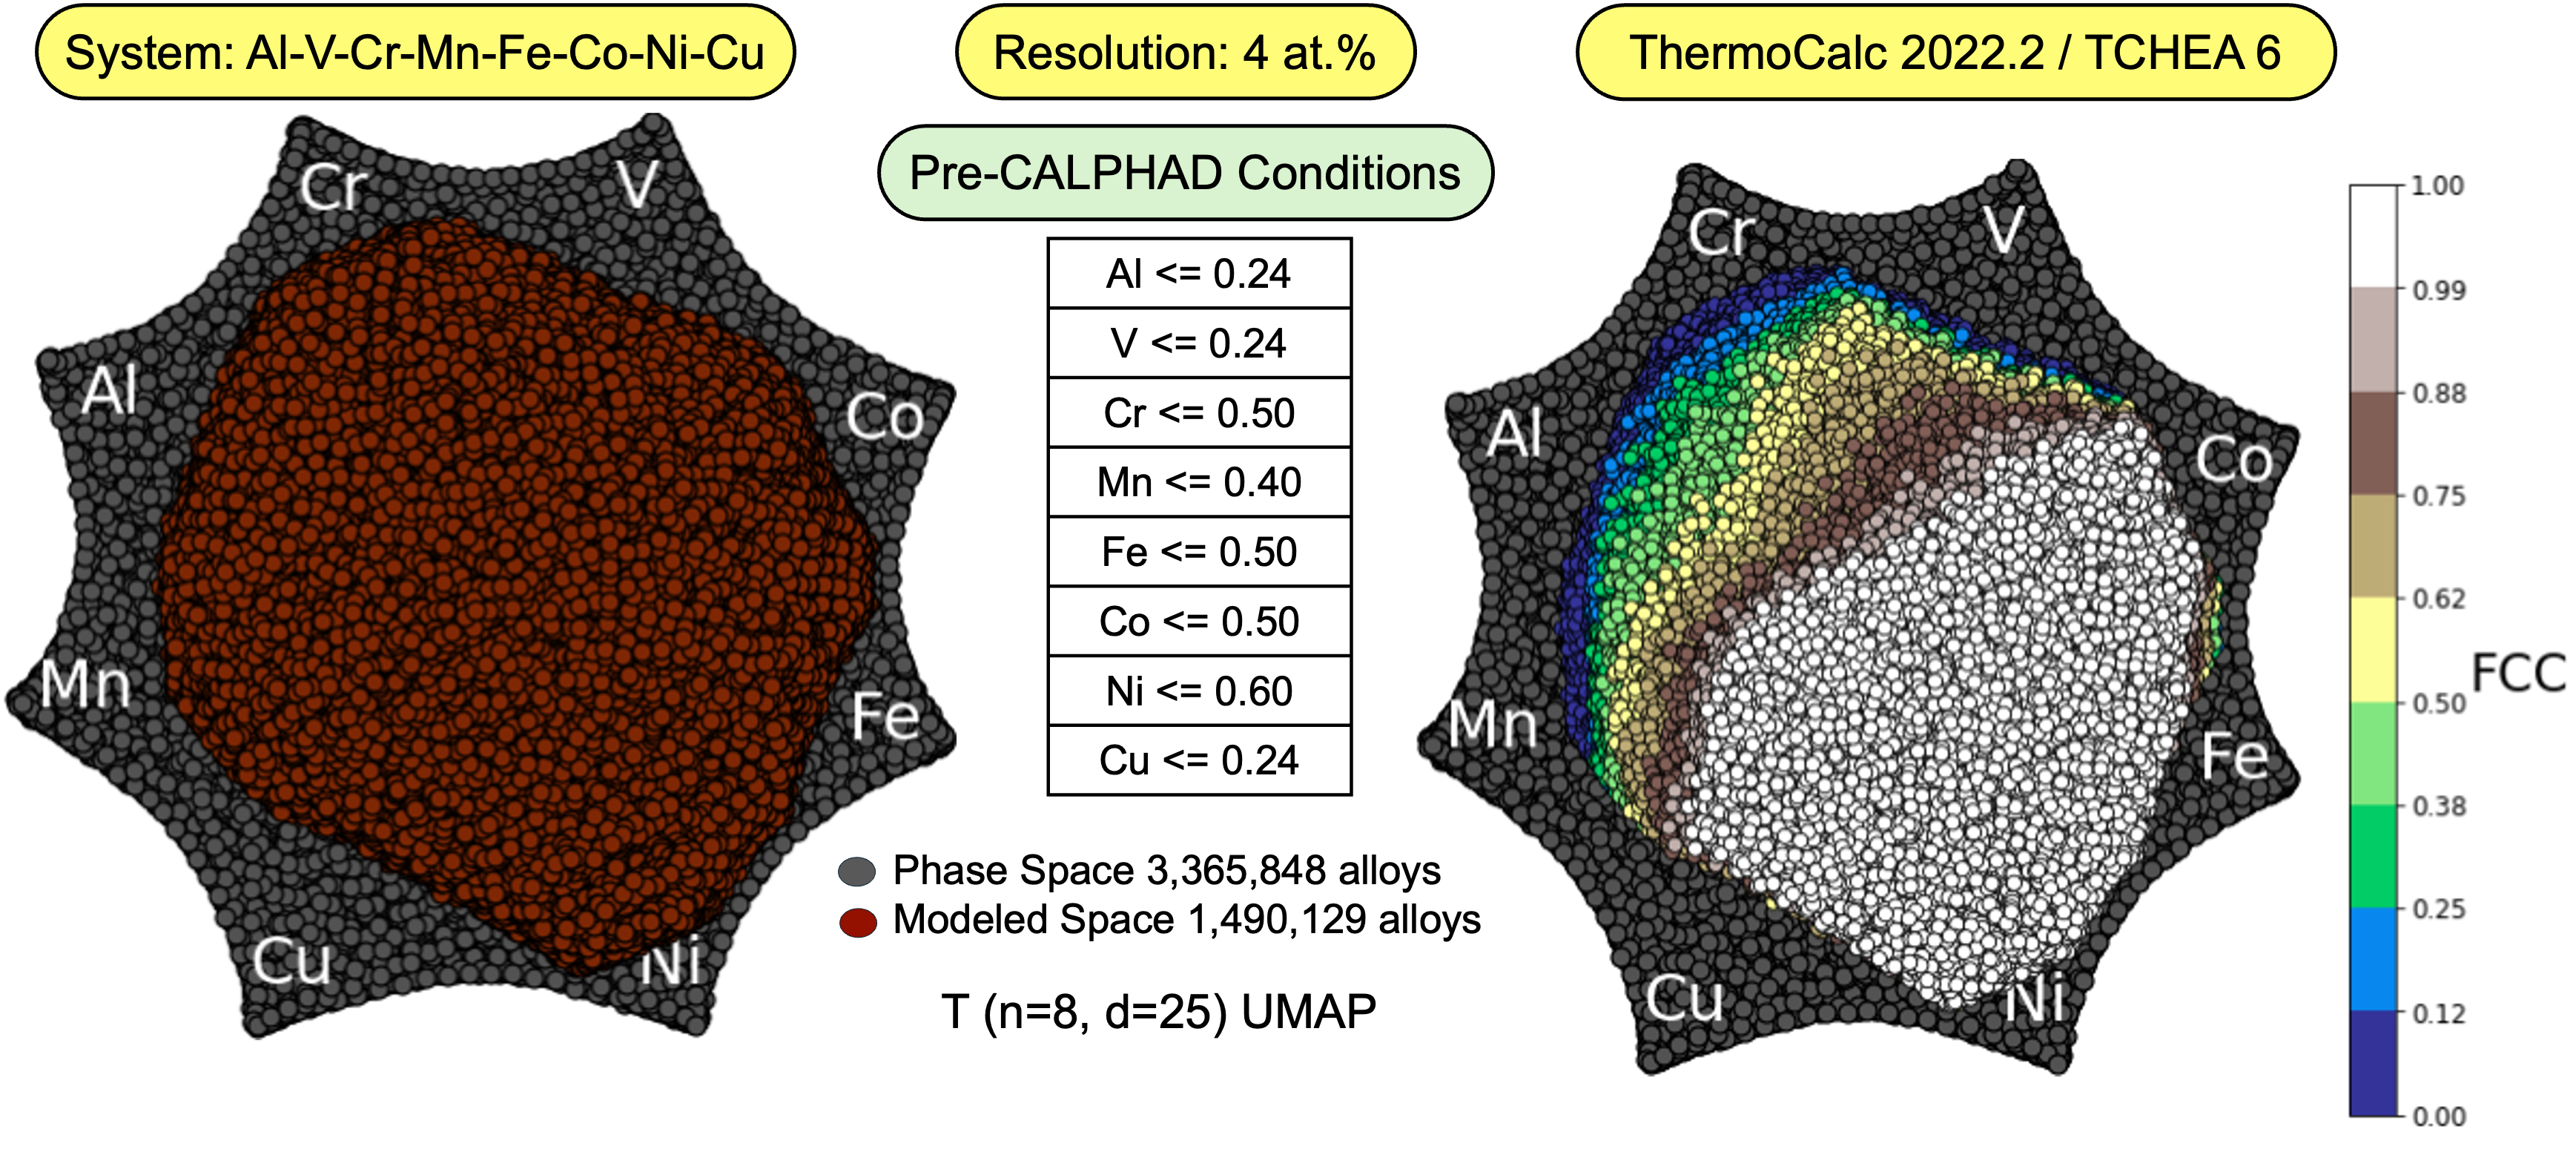
\includegraphics[width=0.8\linewidth]{Figures/feasible_space_v2.png}
    \caption{
    Visualization of the Al–V–Cr–Mn–Fe–Co–Ni–Cu compositional design space and feasible space for this study using UMAP dimensionality reduction. 
    \textbf{(Left)} The full 8-dimensional phase space sampled at 4\,at.\% resolution consists of 3,365,848 possible alloys (gray). \textbf{(Middle)} Expert-imposed compositional maximums, applied to filter for manufacturability, resulting in a reduced modeled space of 1,490,129 alloys (brown).
    \textbf{(Right)} Thermo-Calc (TCHEA6, 2022.2) predictions of FCC phase fraction at 700\textdegree{}C are mapped over the filtered space. Regions with FCC fraction $\geq$ 0.99 (white) define the feasible domain for Bayesian optimization.
    This visualization highlights both the impact of practical compositional constraints and the nonuniform phase stability landscape across the HEA system.
    }
    \label{fig:umap_alloyspace}
\end{figure}



\subsubsection{Candidate Screening via CALculation of PHAse Diagram (CALPHAD) Predictions}

To address the constraint of stabilizing the face-centered cubic (FCC) phase, initial screening of the reduced compositional space is conducted using CALPHAD simulations. CALPHAD method using ThermoCalc has proved to be effective in achieving accurate single phase solid solution predictions and has been demonstrated in for Al-V-Cr-Fe-Co-Ni system \cite{hastings2025acceleratedmultiobjectivealloydiscovery}. In this initial phase, FCC Phase stability of the alloys was predicted using Thermocalc’s TCHEA6 database, to determine compositions that would have a Face-Centered Cubic (FCC) crystal structure (FCC$>$0.99) at 700 °C. By constraining the system with desired material phases and composition maximums, we reduced $\sim$3.36 million compositions into a manageable optimization problem, resulting in a feasible space comprising 26,621 alloys. These constraints effectively narrowed the design space to 0.8 \% of its original size. Several visualizations of downselection are included in \textbf{SI}.  

Subsequently, discrepancies between predicted and experimental phase stability in initial iterations motivated a reanalysis using the updated TCHEA7 database that was released recently. This step was done after iteration BBB, to deal with the challenges that presented along the study. Unlike its predecessor, TCHEA7 enables the prediction of multiple phase regions, specifically FCC, BCC, HCP, SIGMA, and liquid phases, across different temperature regimes. By reevaluating the design space that met the compositional maximums at both 700$^\circ$C and 950$^\circ$C, we ensure that only alloys fully retaining the FCC structure under both conditions are advanced. This dual-temperature screening yields a final feasible set of approximately 27,240 candidate alloys.

\subsubsection{Sampling and Candidate Selection}

Given the large number of candidate alloys resulting from compositional filtering and phase stability screening, an efficient sampling strategy is critical to balance experimental feasibility with adequate coverage of the design space. To explore the feasible space of 26,621 alloys, we implemented a hierarchical sampling strategy using k-medoids clustering. First, the entire feasible space is segmented based on chemical composition into 37 distinct subsystems. These subsystems are defined by the specific combination of elements present (for example, alloys containing all eight elements are classified as System 1, while those with seven elements, are grouped according to their composition and so on). Details of grouping based on subsystems is included in \textbf{SI}.

Subsequently, we apply k-medoids clustering to the feasible space to extract a subset of 1000 representative alloys. In this clustering process, we enforce a constraint that at least one candidate alloy is selected from each of the 37 subsystems, with the number of selections per subsystem proportional to the number of feasible candidates available within that system. This approach guarantees a broad chemical coverage and preserves the diversity of the design space.

From this subset of 1000 alloys, a further down-selection is performed to identify 16 candidate alloys for synthesis. The downselection aims to maximize representation across all 37 subsystems, thereby ensuring that the final batch encapsulates as many distinct chemistries as possible. This diverse and representative sampling is implemented to maximize learning of the complex alloy system and its feasible space by providing a well-distributed training dataset to the Bayesian Optimization (BO) algorithm.


\subsection{Synthesis}

The computationally designed alloys from all iterations were synthesized using high-purity elemental ($>$ 99.9 wt.\%) precursors to produce $\sim$35~g defect-free ingots using Vacuum Arc Melting (VAM) (Edmund B\"{u}hler AM 200) system. The elements were initially melted in Cu crucibles under a high-purity Ar atmosphere. Each ingot was flipped and re-melted 10 times to promote overall uniform chemical homogeneity. Mass loss was monitored throughout processing, and ingots exhibiting losses greater than 0.5\% were reprocessed. Post-solidification, the ingots were homogenized between 950$^\circ$C to 1150$^\circ$C temperature ranges for 24~h in a Centorr LF Series Model~22 high-temperature furnace. The homogenization heat treatment temperatures were selected based on the predicted solidus temperature. Prior to heating, the furnace chamber was purged with Ar gas multiple times to achieve a vacuum of $\sim$5~$\times$~10$^{-5}$~torr. The heat treatment was conducted under a low-pressure Ar atmosphere ($<$10$^{-2}$~torr), followed by furnace cooling.

The homogenized ingots were subsequently cold rolled to a $\sim$60\% reduction in thickness. For recrystallization, the rolled specimens were wrapped in stainless-steel foil with Ti sponge sacrificial getter to minimize oxidation. Recrystallization was performed at 950\textdegree C for 30~min, followed by water quenching to retain the refined fully recrystallized microstructures.

Test sample profiles were precision-cut using wire-Electrical Discharge Machining (EDM). Approximately 4 miniaturized flat tensile specimens, modeled following modified SS-3 designs, were prepared for quasistatic tension testing. Each tensile specimen had a total length of $\sim$26~mm, a gauge length of $\sim$8~mm, and a typical cross-sectional area of 3~$\times$~1~mm$^{2}$, with the loading axis aligned parallel to the rolling direction. Prior to testing, the tensile samples were ground using 120~grit SiC abrasive papers to ensure grip section parallelism, and pinholes were drilled using carbide drill bits. Additional specimens were prepared for microstructural and mechanical characterization, as follows. 2 specimens, each $\sim$2~mm thick with an exposed face area of 8.4~mm$^{2}$ normal to the long rolling direction, were designated for nanoindentation. Another 2 samples, 1.2~mm thick with a face area of 14.4~mm$^{2}$ (also normal to the rolling direction), were allocated for Scanning Electron Microscope (SEM) and Electron Back Scatter Diffraction (EBSD), Energy-Dispersive X-ray Spectroscopy (EDS), X-ray diffraction (XRD), and Vickers hardness (HV) measurements. A schematic of the specimen geometries is shown in Fig.~\ref{fig:Sample Cutting Protocol}.

%To fabricate the designed alloys, high-purity elemental precursors ($>$ 99.9 wt.\%) were used to produce 35 g ingots via vacuum arc melting in an Edmund Bühler AM 200 system. The elements were first melted in copper crucibles under a high-purity argon atmosphere. Each ingot was flipped and re-melted seven times to promote uniform chemical distribution. Throughout synthesis, material integrity was ensured by monitoring weight loss; any ingot exceeding an acceptable threshold was rejected and reprocessed.

%However, incorporating copper and manganese into the compositional space introduced technical challenges. The lower melting points of copper and manganese increased mass loss during fabrication, resulting in more dross formation. Additionally, manganese’s tendency to oxidize required modifying the synthesis process to minimize air exposure. The increased variability in solidus temperatures across compositions also made it difficult to homogenize all samples at the same temperature, adding complexity to the heat treatment process. These factors lengthened the fabrication time and required fine-tuning of the processes.

%Post-synthesis, the ingots underwent homogenization through solution heat treatment at 950°C to 1,150°C for 24 hours in a Centorr LF Series Model 22 high-temperature furnace. The solution heat treatment temperature was decided based on the predicted solidus temperature. Prior to heating, the furnace chamber was purged with argon gas multiple times to achieve a vacuum of 5 × $10^{-5}$ torr. The heat treatment was conducted under a low-pressure argon atmosphere ($<10^{-2}$ torr), followed by controlled slow cooling within the furnace to preserve structural uniformity.

%Following heat treatment, the ingots were subjected to a 60\%\ reduction in thickness via cold rolling. To prepare for recrystallization, the rolled specimens were wrapped in stainless steel foil alongside titanium sponge, which served as a sacrificial getter to minimize oxidation. Recrystallization annealing was carried out at 950°C for 30 minutes, immediately followed by water quenching to retain the refined microstructure.

%Sample profiles were precision-cut using wire electrical discharge machining (wire-cut EDM). Three miniaturized flat tension specimens, modeled after modified SS-3 designs, were prepared for quasistatic tensile testing. Each had a total length of 26 mm, a gauge length of 8 mm, and a typical cross-sectional area of 3 × 1 $mm^{2}$, with the loading axis aligned parallel to the long rolling direction. Additional specimens were prepared for microstructural and mechanical characterization. Two samples, each 2 mm thick with an exposed face area of 8.4 mm² normal to the long rolling direction, were designated for nanoindentation. Another two samples, 1.2 mm thick with a face area of 14.4 $mm^{2}$ (also normal to the rolling direction), were allocated for SEM/EBSD, energy-dispersive X-ray spectroscopy (EDS), X-ray diffraction (XRD), and Vickers hardness measurements.

\begin{figure}[H]
    \centering
    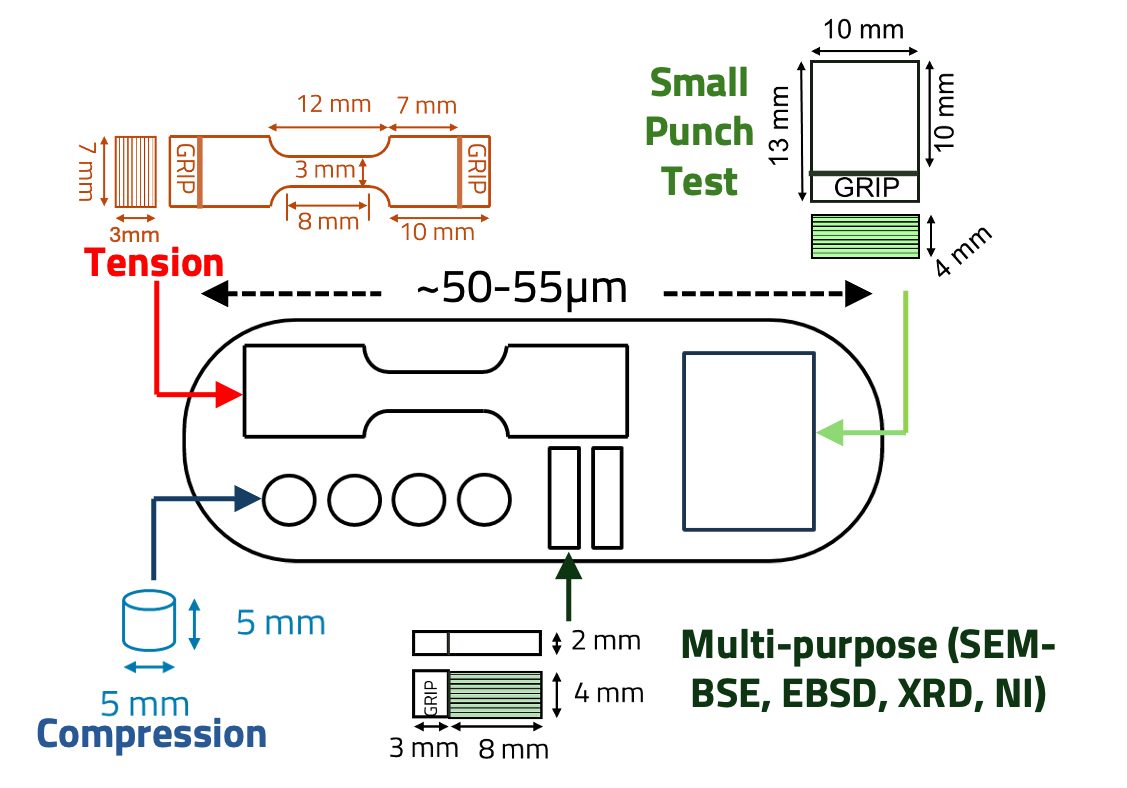
\includegraphics[width=0.6\columnwidth]{Figures/Cutting_Schematic_C2.png}
    \caption{Representative schematics of ingots post-cold rolling with corresponding approximate sample dimensions for distinct characterization tasks: SEM/EBSD, EDS, XRD, and mechanical (Vickers, Nanoindentation) analyses, quasistatic tensile deformation, and Kolsky-bar compression dynamic mechanical response tests.}
    \label{fig:Sample Cutting Protocol}
\end{figure}

In the preparation of the FCC-based high-entropy alloy (HEA) within the Al-Co-Cr-Cu-Fe-Mn-Ni-Mo-V system, it was observed that manganese (Mn) contents exceeding 20 atomic percent introduced significant challenges during arc melting. Mn possesses a relatively low boiling point and a high vapor pressure compared to the other constituent elements, making it highly volatile under the intense localized temperatures generated during arc melting. This volatility leads to substantial Mn evaporation, resulting in deviations from the nominal composition and causing microstructural inhomogeneities and porosity in the cast ingots. The loss of Mn not only disrupts the stability of the intended single-phase FCC structure but also promotes the formation of undesired intermetallic compounds or segregated phases.


%Finally, the tension samples were rough-polished to ensure parallel faces in the grip section, and pinholes were drilled. The $8\cdot4$ and $14\cdot4$ flat samples were then prepared to achieve the high-quality surface required for microscopy techniques and nanoindentation.

\subsection{Verification}

\subsubsection{Metallography}

Microstructural characterization and nanoindentation samples were initially prepared by mechanical polishing using a Buehler AutoMet 250 autopolisher with diamond suspensions down to 1~$\mu$m. For electron backscatter diffraction (EBSD) analysis, the surfaces were subsequently polished to a mirror finish using a Buehler VibroMet 2 vibratory polished for 12~h in a 0.04~$\mu$m colloidal silica suspension. 
%however, sample surfaces were polished using a Buehler Vibromet 2 vibratory polisher, as the surface finish produced by this instrument is not suitable for nanoindentation. The overall surface preparation process is critical to remove distortions, scratches, or embedded debris that could interfere with scanning electron microscopy (SEM) imaging, nanoindentation measurements, and microhardness testing. Key steps in this process include precise mounting, systematic grinding, and final polishing to achieve a flat, mirror-like finish.

In iteration BBA and BBB, samples were individually mounted using graphite mounting powder. Although effective, this method was labor-intensive and caused misalignment during indentation testing in few cases. In addition, it limited batch sizes to eight samples, thereby reducing throughput. To improve efficiency and sample quality, a new preparation technique was developed in iteration BBC. This revised protocol used large aluminum polishing platens that allowed simultaneous processing of 16 or more samples. Samples were fixed to these platens using crystalbond adhesive, ensuring uniform mounting height and eliminating misalignment issues that had previously impacted mechanical characterization. 

To prevent sample mix-ups during high-throughput processing, a laser marking system was introduced. Each sample is lightly marked on its reverse side with a unique identifier indicating the iteration and sample number. Although this step adds to the workflow, it has been optimized for rapid batch processing and ensures reliable traceability throughout testing.

Future plans aim to further increase efficiency by adapting techniques that enable mounting of eight samples per aluminum puck. This adjustment will allow up to 48 samples to be ground and polished concurrently, while maintaining the precise alignment required for subsequent mechanical testing. Overall, these improvements are projected to result in a six fold increase to the sample preparation throughput compared to the initial methods.


\subsubsection{Chemical, Microstructural, and Phase Analyses} 

Compositional analysis was performed using a Tescan FERA-3 Model GMH Focused Ion Beam Microscope equipped with an Oxford energy-dispersive X-ray spectroscopy (EDS) detector, operated at an accelerating voltage of 20 kV. EDS point measurements were obtained from three spatially distinct regions of each processed ingot, with five acquisition points per region and an integrated time of $\sim$50~s per point. The overall composition of each ingot was determined as the arithmetic mean of the 15 measurements. Inter-regional variability was evaluated to assess chemical homogeneity. Representative EDS results from three independent synthesis iterations are presented in Figure \autoref{fig:EDS}. The mean deviation between measured and nominal compositions was $\sim$0.42~at.\%, with 99\% of individual elemental measurements deviating by less than 1~at.\%, indicating a high degree of compositional uniformity.

\begin{figure}[hbt]
    \centering
    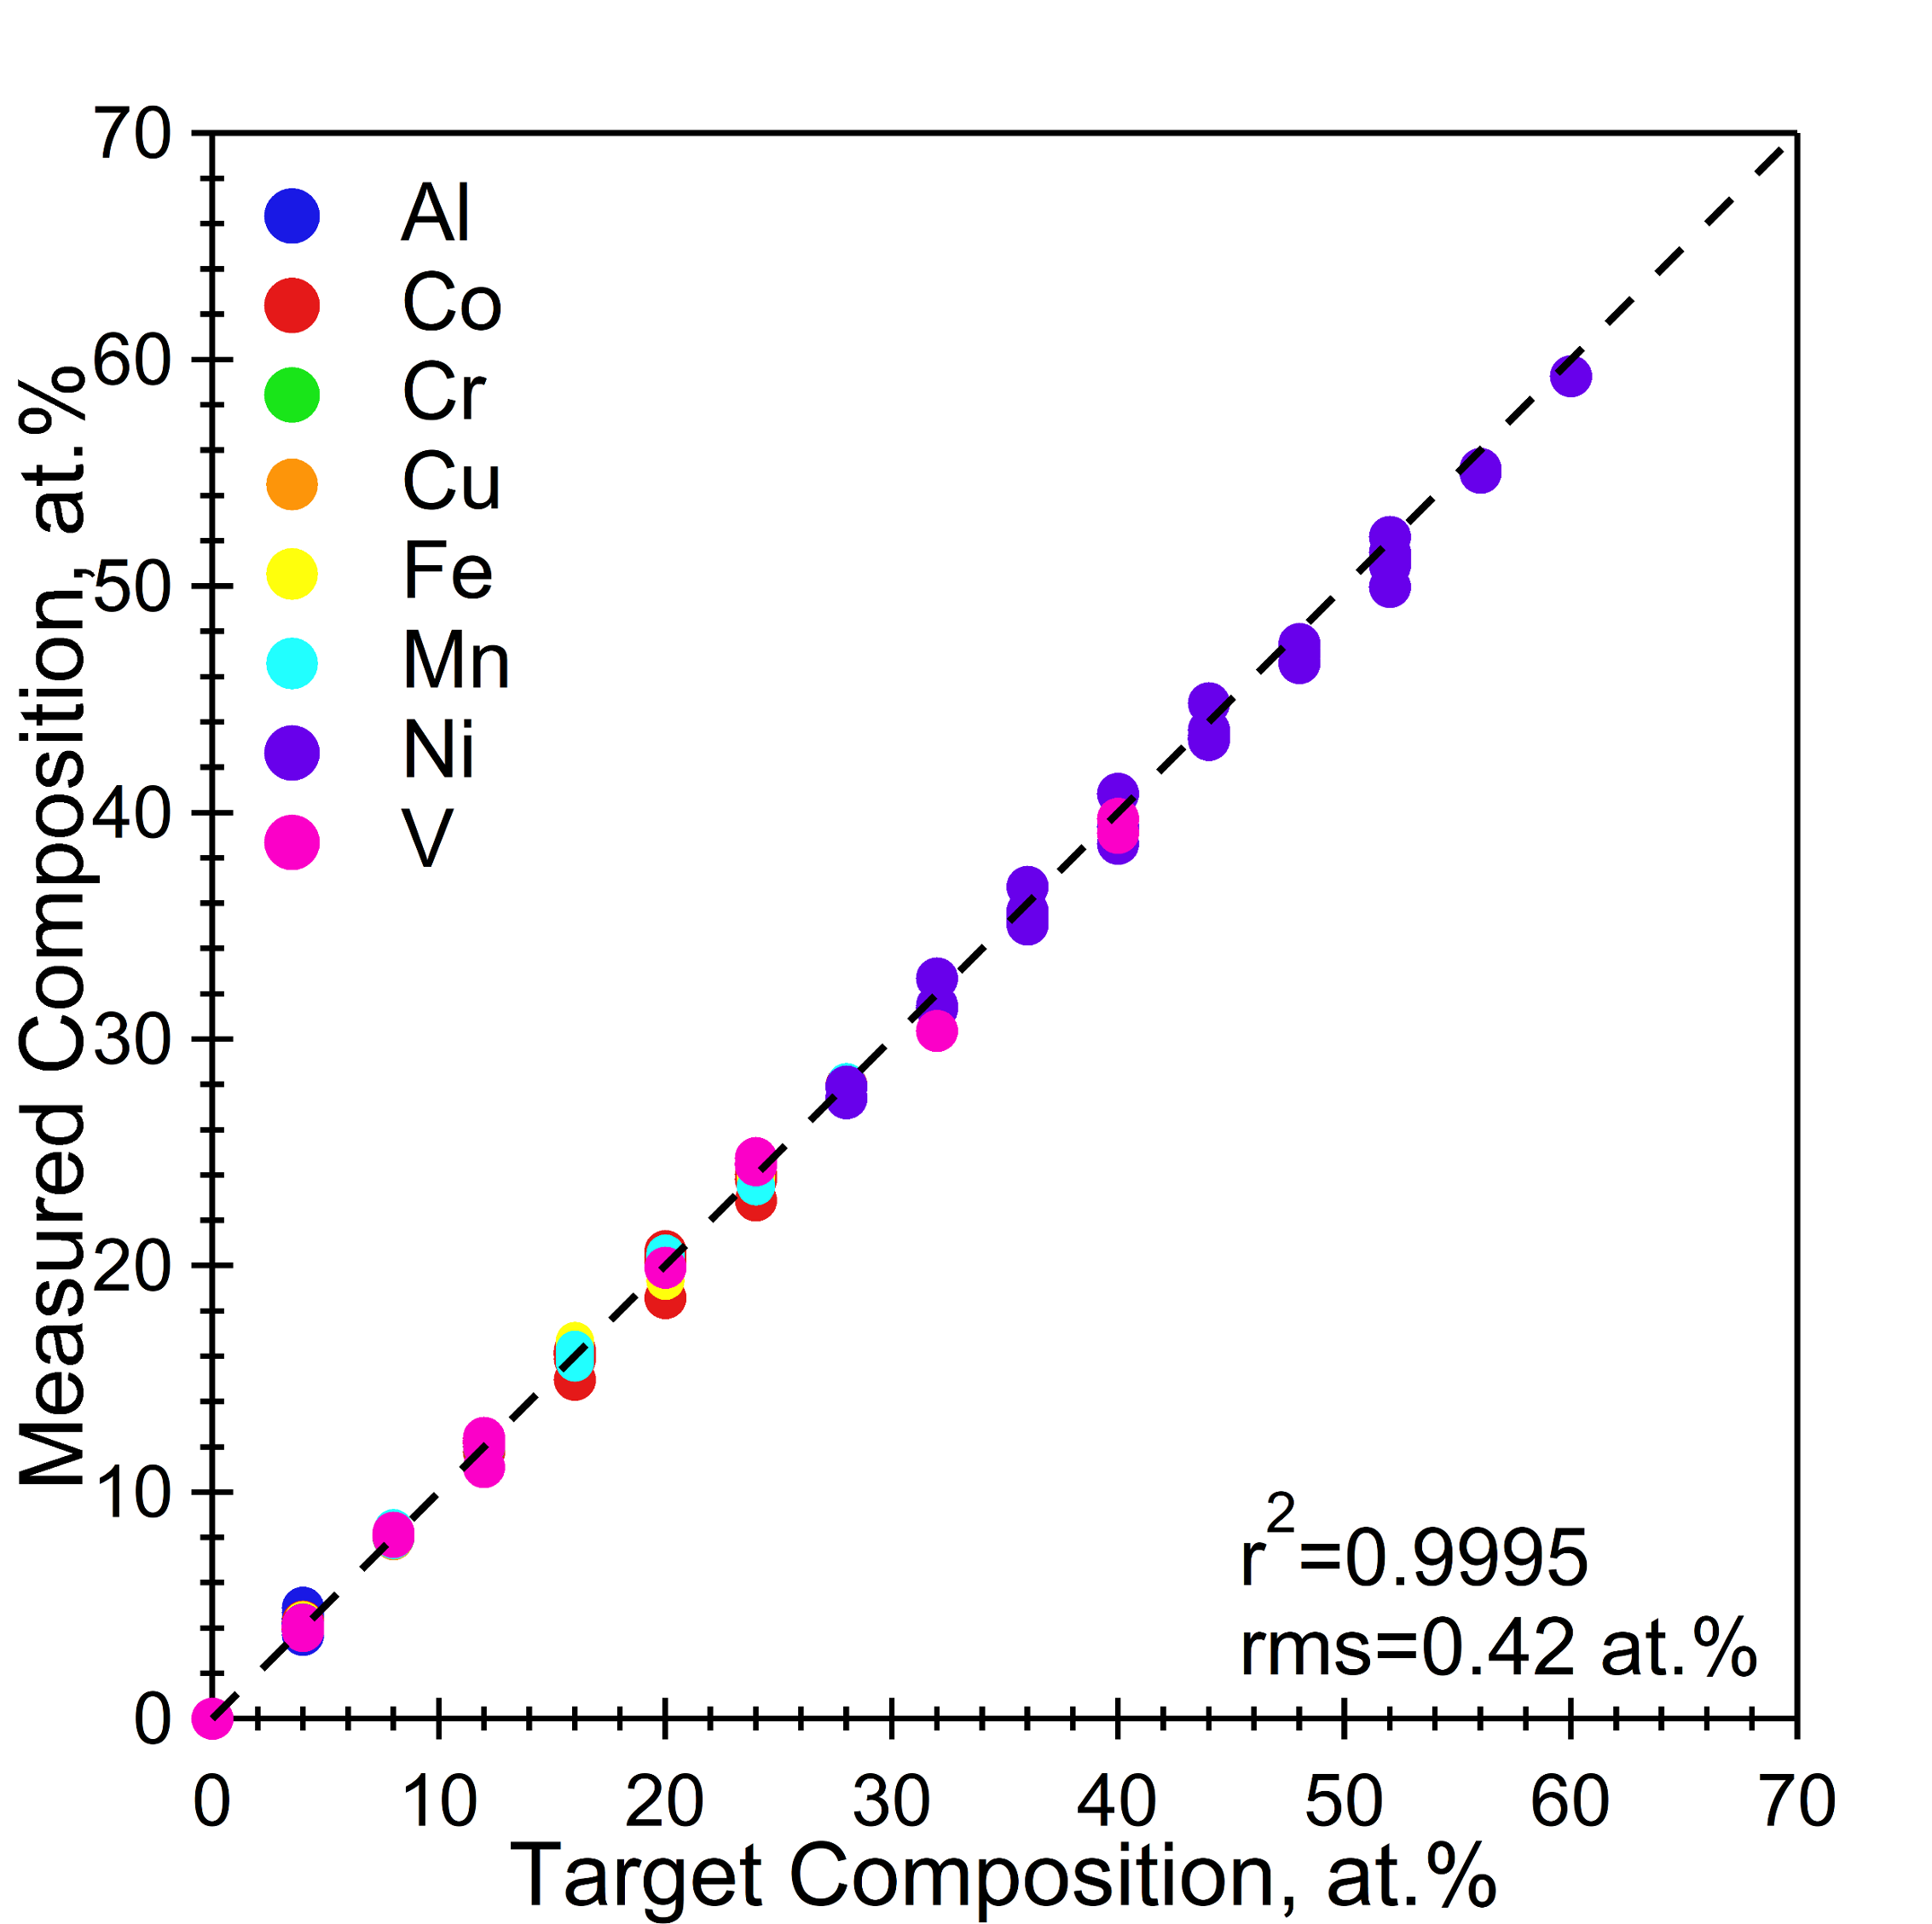
\includegraphics[width=0.3\columnwidth]{Figures/eds_summary.png}
    \caption{Comparison between target and realized chemistry for the samples generated in this study.}
    \label{fig:EDS}
\end{figure}

Microstructural characterization of the undeformed samples was performed by backscattered electron (BSE) imaging at 15~kV using a Phenom XL scanning electron microscope (SEM) with a working distance of $\sim$6~mm. Electron backscatter diffraction (EBSD) measurements were carried out using a FERA SEM equipped with an Oxford Symmetry CMOS-based EBSD detector, operated at an accelerating voltage of 20~kV, a beam current of 18~nA, and a specimen tilt angle of 70$^\circ$. Crystallographic orientation (IPF) maps were acquired on surfaces normal to the cold-rolling direction over an area of approximately 1~$\times$~1~mm$^{2}$, using a step size of $\sim$2~$\mu$m. 

Room-temperature X-ray diffraction (XRD) measurements were conducted using a Bruker D8 Discover diffractometer with Cu K-$\alpha$ radiation ($\lambda$ = 1.5406~\AA) and a 1~mm aperture collimator. Diffraction patterns were collected using a Vantec 500 area detector over a 2$\theta$ range of 30--80$^\circ$. Phase identification and diffraction pattern analysis were performed using the MAUD software package.

%Microstructural characterization of the thermomechanically processed ingots was performed using a FERA scanning electron microscope (SEM). Backscattered electron (BSE) images were acquired from the undeformed alloy surfaces at a working distance of 6 mm. Electron backscatter diffraction (EBSD) was conducted using the same SEM, equipped with an Oxford Symmetry CMOS-based EBSD detector, operated at 20 kV and 20 nA. Crystallographic orientation maps were collected on surfaces oriented normal to the cold rolling direction, covering an area of $1 \times 1 \, \text{mm}$ and a step size of 2 $\mu$m. %The \textbf{SI} includes a collage of representative microscopy images.

\subsection{Characterization} 

\subsubsection{Quasistatic Tensile Deformation} 

Uniaxial tensile tests were conducted at ambient temperature using an MTS 810 servo-hydraulic testing system equipped with an 11.12~kN (2500~lbf) load cell, under a constant quasi-static strain rate of 5~$\times$~10$^{-4}$~s$^{-1}$. Axial strain was measured using an MTS clip-on extensometer mounted directly on the specimen gauge section. An initial force-controlled loading sequence was performed to verify specimen alignment, modulus consistency, and linearity of the elastic response. At least 2 tests were conducted for each condition to ensure reproducibility. Tensile tests were terminated upon complete fracture. True stress--strain ($\sigma$--$\varepsilon$) curves were calculated, from which the ultimate tensile strength (UTS), 0.2\% offset yield strength (YS), and uniform elongation ($\varepsilon$) were determined. These parameters were used to assess the macroscopic tensile mechanical response, as discussed subsequently.

%Isothermal tensile tests were performed using an MTS hydraulic test system equipped with 2500 lbf (11.12 kN) load cell. Tests were conducted at a constant strain rate of \(5 \times 10^{-4} \, \text{s}^{-1}\), with strain measured using an MTS extensometer mounted directly on the specimen gauge section. Each test captured the complete deformation response, from elastic behavior through plastic flow to fracture.  True stress-strain (\(\sigma\)-\(\epsilon\)) curves were generated for each alloy. From these, the UTS and YS at a 0.2\% offset were determined. These values were then used to calculate the strain hardening ratio. 

    
\subsubsection{Nanoindentation} 

Each sample was indented using a KLA Instruments iMicro nanoindenter fitted with a Berkovich diamond tip. Hardness ($H$) and reduced modulus ($E_r$) were determined following the Oliver and Pharr method \cite{Oliver1992}, utilizing $H$ and $E_r$, respectively. %, as outlined in the previous study \cite{hastings2025acceleratedmultiobjectivealloydiscovery}. 

Strain rate jump tests were conducted using nanoindentation to assess the mechanical properties of all designed alloys. These measurements were compared against high strain rate data from the split Hopkinson pressure bar. To improve measurement accuracy, automated methods were developed for quantifying projected contact areas and correcting for pile-up effects, improving the precision of modulus and hardness data.

The automation efforts significantly increased throughput by minimizing manual input during data acquisition and analysis. Custom Python and ImageJ scripts were implemented to automate image acquisition and analysis, addressing one of the primary challenges in establishing an automated system for measuring projected contact area. Ensuring consistent reliability across different materials and strain rates was a critical hurdle that was overcome through iterative refinements.

% \begin{figure}[H]
%     \centering
%     
\includegraphics[width=0.7\columnwidth]{Figures/NI_Automation.png}
%     \caption{Automation of nanoindentation workflows to increase throughput of NI analysis.}
%     \label{fig:SRJT_NI}
% \end{figure}

These improvements also facilitated direct comparisons between nanoindentation data and results from high strain rate methods, such as the split Hopkinson pressure bar. The strain rate sensitivities obtained from these different techniques were found to be in close agreement, typically within one standard deviation. The advanced automation and streamlined workflow have laid the groundwork for more accurate and high-throughput mechanical testing across varying strain rates, thereby helping understand the material behavior during deformation while enhancing the overall efficiency of the experimental process.


\subsubsection{High Strain Rate Nanoindentation}

In this study, nanoindentation instrument to measure hardness during high strain rate indentation impact testing, allowing one to assess hardness at strain rates exceeding \(10^{3}~\text{s}^{-1}\), has been adapted. Nanoindentation impact tests were conducted using an indenter system that contains a hexapod specimen stage and an InForce 1000 actuator that has been customized to measure displacements at high acquisition rates using a Michelson interferometer. More details of this setup can be found in \cite{Hackett2023}. All tests were conducted with a Berkovich three-sided pyramid tip.

Quasistatic constant indentation strain rate tests were performed using a constant \(\frac{\dot{P}}{P}\) test (force rate over force) with a target \(\frac{\dot{P}}{P} = 0.2~\text{s}^{-1}\) and a target load of 1~N. Dynamic tests consisted of indentation impact tests with an impact force of 20~mN followed by a re-loading at the same indent location up to a load of 1~N at a target \(\frac{\dot{P}}{P} = 0.2~\text{s}^{-1}\). The purpose of this re-loading was to attempt to evaluate and compare the dynamic to quasistatic hardness ratio, \(\frac{H_{\text{DYN}}}{H_{\text{QS}}}\), as obtained from separate tests with those obtained from a single testing point. The results from this will be presented in a separate study.

The hardness was evaluated at a depth of 2000~nm. This was done by taking the load at 2000~nm and dividing it by the expected projected contact area at this depth. The expected projected contact area was calculated using the area function of the tip, \(A(h)\), which was found by a separate calibration procedure on fused silica \cite{Oliver1992}, and evaluating it at the contact depth, \(h_c\). The contact depth at 2000~nm was found by multiplying this indentation depth with the contact depth to indentation depth ratio, \(h_c/h\). The contact depth to indentation depth ratio was found by imaging each indentation contact impression after testing and finding the residual and nominal contact areas, \(A_R\) and \(A_N\), respectively, by tracing the impressions manually in images from a laser confocal microscope and thresholding the images to obtain the nominal contact area. The ratio was then estimated as \(h_c/h = \sqrt{A_R/A_N}\).


An analysis code was developed to streamline data collection and export, optimizing the workflow for high-throughput analysis. The hardness of designed high entropy alloy compositions at high strain rates (10³ s\(^{-1}\)) and low strain rates (2 s\(^{-1}\)) was measured, quantifying their rate sensitivities by comparing the hardness values at both strain rates. Details on this method are provided in the Supplemental Material. This capability significantly contributed to the ability to characterize material performance under extreme conditions.




Integrating the high strain rate nanoindentation system into our workflow had several technical challenges. The instrument outputs data in encrypted binary files, which requires development of Python scripts for reliable data extraction. Efforts were dedicated to optimizing these scripts for user-friendliness and automating quantifying the projected contact area of residual impressions. %These enhancements were critical for improving efficiency and ensuring precise data analysis.
As a result, high strain rate hardness data was successfully acquired for all candidate alloy compositions and incorporated into the Bayesian optimization loop. Further automation scripts were developed to handle complex data analysis tasks, reducing processing time. Additionally, nanoindentation data was cross-validated with tensile and Hopkinson bar test results to identify correlations in rate sensitivity across the three measurement techniques. The rate sensitivities from all methods were found to be within one standard deviation of each other.


% \subsubsection{Small Punch Test}

% In addition to quasistatic tensile tests, Small punch test was intended to measure the dynamic response of materials in this study and modified Split Hopkinson Pressure Bar (SHPB) design was selected due to its ability to minimize uncertainty during testing. In this configuration, the output bar serves as the SPT indenter, while the input bar secures the sample, which incorporates a central hole to accommodate the passage of the indenter.

% To optimize the setup, existing CAD designs were refined to enhance the sample holding mechanism and improve data acquisition. A virtual experiment was conducted using ABAQUS finite element analysis to simulate the SHPB setup, ensuring material compatibility and minimizing wear. This virtual modeling was instrumental in expanding the testing capability to a wide range of metallic materials. Strain gauges were  chosen for data acquisition due to their established reliability and ease of integration. Another critical challenge was achieving uniform uniaxial stress on the sample, complicated by the presence of the central hole in the input bar. Iterative modifications addressed these issues, resulting in a more robust experimental design and improved data quality.

% For Small Punch Test (SPT) to evaluate the mechanical response of the HEA samples, plate-shaped specimens were extracted from the grip section of the tensile specimen created from VAM-processed buttons and prepared for testing. Each plate was carefully ground to a uniform thickness of approximately 500~µm using successive grades of silicon carbide (SiC) abrasive paper to ensure surface flatness and reduce surface artifacts that could influence test results.

% \emph{Experimental Details:} The SPT samples were tested using a standardized test fixture consisting of a lower die with a 4mm diameter circular opening and a hemispherical punch of 2.4mm diameter. The die and punch were precisely aligned to ensure concentric loading, and the sample was clamped securely between the upper and lower fixtures to minimize tilting or lateral motion. To reduce frictional effects and ensure repeatability, a thin layer of Silicon oil lubricant was applied between the punch and the specimen surface prior to testing.

% The tests were conducted on a Zwick-Roell universal testing machine equipped with a 2.5kN load cell. The punch was driven vertically at a constant displacement rate of 0.3mm/min until complete rupture of the specimen occurred. Load–displacement data were continuously recorded during each test for subsequent analysis and inverse modeling. The alignment and fixturing procedure were repeated identically across all specimens to maintain consistency in test conditions.

% \begin{figure}[htbp]
%     \centering
%     \begin{subfigure}[b]{0.3\textwidth}
%         \includegraphics[width=\textwidth]{Figures/Spt_schematic.png}

%     \end{subfigure}

%     \caption{Schematic of SPT experiment}
%     \label{fig:spt_config}
% \end{figure}

% \emph{Analysis:} To enable uncertainty-aware inference of elastic–plastic material parameters from Small Punch Test (SPT) data, we adopt a recently developed Bayesian framework \citep{} that integrates: (1) a Gaussian Process Regression (GPR) surrogate trained on finite element (FE) simulations, (2) a model discrepancy correction term to account for systematic mismatches between simulations and experimental data, and (3) Markov Chain Monte Carlo (MCMC) sampling to infer posterior distributions over material parameters.

% The Bayesian framework is structured to allow sequential determination of material properties: the unloading region is used to infer the elastic modulus, while the plastic parameters are extracted from the loading segment corresponding to initial contact, plastic bending, and membrane stretching. These deformation regimes are identified based on changes in the slope of the load–displacement curve, which serve as indicators of transitions in the dominant mechanical response. By isolating and analyzing the most informative segments, the protocol improves parameter identifiability and enhances the physical interpretability of the inference process.

\subsubsection{Split-Hopkinson Pressure Bar (SHPB) test}

To characterize the high strain rate mechanical behavior of the high-entropy alloys (HEAs) developed in this program, Split-Hopkinson Pressure Bar (SHPB) testing was performed on all candidate alloys. For each composition, a minimum of two specimens were tested, and approximately half of the alloys were evaluated at multiple strain rates, namely 1500\,s$^{-1}$ or both 1500\,s$^{-1}$ and 3000\,s$^{-1}$. 

The SHPB experiments employed a pulse-shaping technique to achieve and maintain a uniform strain rate throughout the major portion of the specimen deformation. A Ni-30Mo alloy was used as the pulse shaper due to its strain hardening behavior, which closely resembles that of the tested HEAs. The SHPB setup captures three essential waveforms: the incident pulse, transmitted pulse, and reflected pulse. %An example of these signals is shown in \autoref{fig:shpb_signals} on left. The shaped incident pulse (green curve in the negative time quadrant) initiates loading of the sample. The first red waveform in the negative quadrant corresponds to the transmitted signal, from which the stress-time history is obtained. The green waveform in the positive quadrant represents the reflected pulse, which is integrated over time to calculate the strain-time profile.

These signals are time-synchronized to construct the dynamic stress–strain response of the material. \autoref{fig:shpb_signals} shows representative results from two SHPB tests performed at a nominal strain rate of 1500\,s$^{-1}$. The black curves represent the true engineering stress–strain response, while the blue curves illustrate the instantaneous strain rate as a function of strain. This methodology enabled reliable and high-fidelity characterization of dynamic mechanical behavior across the HEA compositions, forming a critical component of the multi-objective optimization framework.

\begin{figure}[H]
    \centering
    \includesvg[width=0.5\linewidth]{Figures/SPHB2.svg}
    \caption{Dynamic engineering stress–strain responses (black) and corresponding strain rate as a function of strain (blue) for two HEA samples tested at 1500\,s$^{-1}$.}
    \label{fig:shpb_signals}
\end{figure}


%\subsubsection{LIPIT} - not used in BO

\subsection{Depth of Penetration Simulation}

\emph{Viscoplasticity Constitutive Model Implementation:} The ballistic impact response of the high entropy alloys was modeled using the Cowper-Symonds (CS) viscoplasticity constitutive framework to capture the inherent strain rate sensitivity exhibited by these materials under dynamic loading conditions. The CS model provides a description of the flow stress evolution as a function of plastic strain rate through a multiplicative enhancement factor applied to the quasi-static flow strength. The constitutive relationship is expressed as:

\begin{equation}
\sigma_f = \sigma_{qs}^f \left(1 + \left(\frac{\dot{\varepsilon}_p}{C}\right)^{1/m}\right)
\end{equation}

where $\sigma_{qs}^f$ represents the quasi-static flow strength that evolves with accumulated plastic strain due to work hardening mechanisms, $\dot{\varepsilon}_p$ denotes the effective plastic strain rate, $C = 10^3 \text{ s}^{-1}$ serves as a material-dependent constant multiplier, and $m$ constitutes the strain rate sensitivity exponent within the CS formulation. This multiplicative formulation enables the model to account for the dynamic strengthening observed in high entropy alloys under high strain rate deformation, where dislocation motion becomes increasingly constrained at elevated loading rates.

\emph{Rate Sensitivity Parameter Identification:} The strain rate sensitivity parameter $m$ for each high entropy alloy composition was determined using a systematic calibration procedure utilizing experimental data obtained from quasistatic uniaxial tension tests and dynamic SHPB compression experiments conducted at strain rates ranging from $10^{-3} \text{ s}^{-1}$ to $10^4 \text{ s}^{-1}$. The parameter identification process employed a nonlinear least-squares optimization algorithm to minimize the root mean squared error (RMSE) between the CS model predictions and experimental true stress measurements:

\begin{equation}
\text{RMSE} = \sqrt{\frac{1}{N}\sum_{i=1}^{N}\left(\sigma_{pred,i}^f - \sigma_{obs,i}^f\right)^2}
\end{equation}

where $N$ represents the total number of discrete data points in the experimental stress-strain response, $\sigma_{pred,i}^f$ denotes the model-predicted flow stress at the $i$-th data point, and $\sigma_{obs,i}^f$ corresponds to the experimentally observed true stress value. The optimization procedure was implemented under isothermal conditions to isolate the strain rate effects from thermal softening mechanisms. The calibrated rate sensitivity exponents for the investigated high entropy alloy compositions ranged between 2 and 6, consistent with the expected strain rate sensitivity behavior of face-centered cubic polycrystalline materials.

\emph{Finite Element Ballistic Impact Simulation:} The calibrated material parameters were subsequently implemented into a user-defined material subroutine (UMAT) within the ABAQUS/Explicit finite element framework to simulate the ballistic impact response. The computational model employed a two-dimensional axisymmetric formulation to simulate the normal impact of a rigid spherical projectile onto a cylindrical target fabricated from the characterized high entropy alloy. The target geometry consisted of a cylinder with radius $r_t = 25$ mm and thickness $t = 16$ mm, while the projectile was modeled as a rigid sphere with diameter $d_p = 10$ mm impacting at a velocity of $V_0 = 500$ m/s.

The finite element discretization utilized explicit, linear, axisymmetric stress elements (CAX3R) with a characteristic mesh size of 0.5 mm, resulting in a computational domain of 30 × 51 elements in the radial and axial directions, respectively. The target material properties included an elastic modulus $E_t = 200$ GPa, Poisson's ratio $\nu_t = 0.3$, and density $\rho_t = 8.75 \times 10^{-6}$ ton/mm³. Mesh distortion controls were implemented using default ABAQUS settings, with future work planned to incorporate adaptive remeshing algorithms to maintain solution accuracy throughout the large deformation impact event.

\emph{Depth of Penetration Quantification:} The ballistic performance of each high entropy alloy composition was quantified through the depth of penetration (DoP) metric, defined as the maximum axial displacement of the projectile centroid into the target material during the impact event. The DoP measurement was extracted from the finite element solution at the instant of maximum penetration, typically corresponding to the time when the projectile velocity approaches zero. This performance metric provides a direct quantitative assessment of the material's ballistic resistance capability and serves as the primary response variable for correlating material properties with impact performance. The DOP values were recorded with sub-millimeter precision from the simulation output, enabling detailed statistical analysis of the property-performance relationships across the investigated compositional space. DoP was extracted as the maximum penetration depth reached by the projectile, tracked over the course of the simulation. Alloys from multiple optimization iterations were evaluated under identical loading conditions using calibrated viscoplastic constitutive models.

% \begin{figure}[H]
%     \centering
%     
\includegraphics[width=1\linewidth]{Figures/dop determ.PNG}
%     \caption{(Left) Example simulation at four different timestamps, where (a) is the first point of contact, (c) is the maximum DOP, and (d) is the post-impact damage. (Right) Graph depicting the displacement of the contact point between projectile and target.}
%     \label{fig:FindDoP}
% \end{figure}


%\subsection{Performance Objectives}

% \subsection{Integration of Experimental/Simulation Outputs of Objectives into the Bayesian Optimization Loop}

% Having established the alloy design pipeline, defining an 8‑dimensional compositional grid, applying CALPHAD‑based phase filters, and selecting candidates via diversity‑aware k‑medoids sampling, initial batch of 16 alloys were synthesized using vacuum arc melting (VAM). Each ingot was subjected to rigorous metallographic, chemical, and microstructural verification (SEM, EBSD, EDS, XRD) to confirm phase purity and homogeneity as discussed above. Subsequently, we characterized their mechanical response under both quasi‑static and dynamic loading conditions: uniaxial tensile tests provided yield strength (YS), ultimate tensile strength (UTS), UTS/YS ratio, and engineering strain at UTS; instrumented nanoindentation with strain rate jump protocols yielded hardness and strain rate sensitivity; high‑strain‑rate nanoindentation and split Hopkinson pressure bar tests quantified dynamic strength. %; and dynamic small punch testing (SPT) offered complementary miniaturized high‑rate deformation data. 
% In parallel, finite element simulations of Kolsky bar impacts delivered depth of penetration (DoP) predictions as a surrogate for impact resistance.

% As discussed before, these five key metrics were selected as optimization objectives in the Bayesian loop. 
% % \begin{enumerate}
% %   \item \textbf{Yield Strength (YS)}: a primary indicator of the alloy’s resistance to permanent deformation under service loads.
% %   \item \textbf{UTS/YS Ratio}: reflecting the strain hardening capacity and the balance between strength and ductility.
% %   \item \textbf{Engineering Strain at UTS} ($\varepsilon_\text{UTS}$): Capturing the fracture strain at peak load, a direct measure of ductility.
% %   \item \textbf{Dynamic to Quasi‑Static Strength Ratio} ($\sigma_\text{dyn}/\sigma_\text{qs}$): quantifying strain‑rate sensitivity by comparing SHPB (and high‑rate nanoindentation) results to quasi‑static tensile strength.
% %   \item \textbf{Depth of Penetration} (DoP): included as a minimization objective to favor alloys with superior impact resistance.
% % \end{enumerate}
% These objectives collectively capture the performance required for demanding structural applications, from low‑rate load bearing to high‑rate impact scenarios.

% These experimental and simulation outputs are integrated into a \emph{batch Bayesian optimization} (BO) framework that iteratively refines Gaussian process surrogate models for each objective. In each iteration, the Expected Hypervolume Improvement (EHVI) acquisition function proposes a new batch of 16 alloy compositions to maximize the multi‑objective gain. A \textbf{risk-aware strategy} is used to handle phase stability and manufacturability constraints: candidate alloys that violate the FCC single phase requirement, or candidates associated with manufacturing difficulty, are not strictly excluded but are assigned lower sampling priority, ensuring critical exploration around phase‑boundary regions without introducing undue bias.

% As new alloys are synthesized and characterized, their measured YS, UTS/YS, $\varepsilon_\text{UTS}$, $\sigma_\text{dyn}/\sigma_\text{qs}$, and DoP data are fed back into the BO loop, updating the surrogate models. Through this closed‑loop process, current study systematically identifies the Pareto‑optimal set of FCC HEAs, balancing strength, ductility, rate sensitivity, and impact resistance while respecting manufacturability and phase stability considerations.

% \begin{figure}[H]
%   \centering
%   
\includegraphics[width=\linewidth]{Figures/HTP_synthesis_characterization.png}
%   \caption{
%     High‑throughput synthesis and characterization workflow for the current study. The five objectives (YS, UTS/YS ratio, strain@UTS, dynamic/quasi‑static strength ratio, and DoP) feed back into the batch Bayesian optimization loop, guided by an EHVI acquisition and a probabilistic phase‑stability classifier.
%   }
%   \label{fig:pipeline}
% \end{figure}

% As shown in \autoref{fig:pipeline}, all experimental measurements and simulation outputs are integrated as surrogate‐model training data, driving each subsequent BO batch toward the Pareto front under a risk‑aware, multi‑objective framework.


\subsection{Computational Design Framework}

Our closed-loop design framework consists of multiple ingredients that each introduce a unique capability to the framework. In the following, each part of the framework is introduced in detail, and we explain how these parts are integrated to enable accelerated design using the Bayesian approaches.


\subsubsection{Gaussian Process Regression}

Bayesian optimization is established because of the capability to represent expensive-to-evaluate black-box objective functions using surrogate models. A surrogate model is a cheap source for predicting the outcomes of yet to be observed experiments to feed a utility value function for decision-making purposes. In such a scenario, a probabilistic model can provide uncertainty-aware predictions so that the decisions are made considering the probability of observing different outcomes of the same experiment. One such probabilistic model is Gaussian process regression which is used for modeling in various fields due to its low computational costs~\cite{Rasmussen:2005:GPM:1162254}. GP predictions rely on the distance-based correlation between data points and it is a flexible model which can be easily manipulated to suit the modeling requirements of different applications.

Assuming there are $N$ previously observed data denoted by $\{\mathbf{X}_{N}, \mathbf{y}_{N}\}$, where $\mathbf{X}_{N} = (\mathbf{x}_{1}, \ldots, \mathbf{x}_{N})$ and $\mathbf{y}_{N} = \left(f(\mathbf{x}_{1}), \ldots, f(\mathbf{x}_{N})\right)$, then the GP probabilistic prediction at unobserved location \textbf{x} is a normal distribution:
\begin{equation}
\label{GP11}
f_{\textrm{GP}}(\mathbf{x}) \mid \mathbf{X}_{N}, \mathbf{y}_{N} \sim \mathcal{N}\left(\mu(\mathbf{x}),\sigma_{\textrm{GP}}^2(\mathbf{x})\right)
\end{equation}
where
\begin{equation}
\begin{aligned}
\label{meancov}
\mu(\mathbf{x}) &= K(\mathbf{X}_{N},\mathbf{x})^\textrm{T}[K(\mathbf{X}_{N},\mathbf{X}_{N})+\sigma^2_{n}I]^{-1} \mathbf{y}_{N}\\
% \sigma_{\textrm{GP}}^2 (\mathbf{x})  &=  k(\mathbf{x},\mathbf{x}) - K(\mathbf{X}_{N},\mathbf{x})^\textrm{T} \\
% &\qquad \quad [K(\mathbf{X}_{N},\mathbf{X}_{N})+\sigma^2_{n}I]^{-1}K(\mathbf{X}_{N},\mathbf{x})
\sigma_{\textrm{GP}}^2 (\mathbf{x})  &=  k(\mathbf{x},\mathbf{x}) - K(\mathbf{X}_{N},\mathbf{x})^\textrm{T} [K(\mathbf{X}_{N},\mathbf{X}_{N})+\sigma^2_{n}I]^{-1}K(\mathbf{X}_{N},\mathbf{x})
\end{aligned}
\end{equation}
here, $k$ is a real-valued kernel function to calculate correlations, $K(\mathbf{X}_{N},\mathbf{X}_{N})$ as a $N \times N$ matrix with $m,n$ entry as $k(\mathbf{x}_{m}, \mathbf{x}_{n})$, and $K(\mathbf{X}_{N}, \mathbf{x})$ is a $N \times 1$ vector with $m^{th}$ entry as $k(\mathbf{x}_{m}, \mathbf{x})$.  The term $\sigma^2_{n}$ is used to model experiment errors. A common choice for kernel function is squared exponential:
\begin{equation}
\label{eq:5}
k(\mathbf{x},\mathbf{x'}) = \sigma_s^2 \exp\left(- \sum_{h = 1}^{d} \frac {(x_h-x'_h)^2}{2l_h^2}\right )
\end{equation}
where $d$ is the dimensionality of the input space, $\sigma_s^2$ is the signal variance, and $l_h$, where $h = 1,2,\ldots,d$, is the characteristic length-scale to determine correlation strength between data points within dimension $h$.

\subsubsection{Informative Priors for Gaussian Process Regression}

Typically, a GPR mean function is initially set to zero, disregarding the opportunity to incorporate valuable prior knowledge into the model. In some cases, the mean function is shifted so a GPR defaults to the average of training data as the best prediction if no observation is available. One approach to incorporate prior knowledge in the presence of a prior model in constructing a GPR is to augment the prior model as the GPR mean function, which we call a GPR with \textit{informative prior}. Then, it is trained with experimental observations to override the prior model predictions, but it defaults to the prior model predictions at regions with no observations. Mathematically, a GPR with an informative prior is built over the discrepancy between the prior model and the experimental observations. Note that if $f\sim \textrm{GP}~(\mu,k)$, then $f'=f-\mu$ is a zero mean GP. Thus, a zero mean GP is constructed to represent the discrepancy between experimental observations and prior, $f'$, and prior, $\mu$, is added to $f'$ to obtain posterior on $f$. This approach guarantees that a GPR override prior if observations exist, else, exploits prior for probabilistic modeling.

In this work, we employ GPR with an informative prior to develop a machine learning model that integrates physical insights from the Varvenne–Luque–Curtin solid solution strengthening model \cite{varvenne2016theory} as the prior, \(\mu\). This model captures the strengthening behavior of FCC high entropy alloys (HEAs) by accounting for solute misfit volumes, modulus mismatch, and local lattice distortions in a fully random solution. We combine this physics-based prior with limited experimental data, including Vickers hardness (HV) and temperature-dependent yield strength (YS) measurements.

Let the true composition temperature dependent mechanical behavior of the HEAs be denoted by the function \(f_{\textrm{exp}}(\mathbf{x})\), where \(\mathbf{x}\) is a vector describing the alloy composition and test temperature. The GPR model is built over the residual (or discrepancy) between experimental observations and the prior prediction, defined as \(f_{\textrm{dis}}(\mathbf{x}) = f_{\textrm{exp}}(\mathbf{x}) - \mu(\mathbf{x})\). The final GPR prediction, which combines the data-driven discrepancy model with the physically-informed prior, is then expressed as:
\[
f(\mathbf{x}) = f_{\textrm{dis}}(\mathbf{x}) + \mu(\mathbf{x}).
\]


The machine learning models were developed using data from \cite{hastings2025acceleratedmultiobjectivealloydiscovery} in conjunction with the {\tt CBFV}~\cite{Murdock2020IsProperties} and {\tt HEACalculator} packages~\cite{doguhan_sariturk_2022_7429046} for composition feature generation. These tools generated over 5000 features for each composition, which were subsequently optimized using the RecursiveByShapValues method~\cite{Prokhorenkova2018CatBoost:Features} to eliminate redundant features based on SHAP (SHapley Additive exPlanations) values. Given the tabular nature of the dataset, with a limited number of datapoints and a high dimensionality of features, the CatBoost gradient boosting algorithm~\cite{Prokhorenkova2018CatBoost:Features} was utilized.

\subsubsection{Probability‑Aware Design Strategy}

To systematically incorporate phase stability constraints into our multi-objective optimization, we employ a \textbf{Gaussian Process Classifier (GPC)} to model the feasibility of candidate alloys. The GPC is trained on an initial dataset of alloys labeled as \textit{feasible} (FCC phase fraction $>$ 0.99 at both 700\textdegree C and 950\textdegree C) and \textit{infeasible} (alloys with secondary phases). Rather than deterministically excluding designs near the stability boundary, we use the GPC’s probabilistic output, $P_\text{feas}(x)$, to softly penalize—but not eliminate—candidates with lower predicted feasibility. 

Candidates with $P_\text{feas}(x) \geq 0.8$ are retained in the Expected Hypervolume Improvement (EHVI) acquisition process, allowing the framework to continue exploring regions of uncertainty if they show promise in the multi-objective landscape. The classifier is updated iteratively as new alloys are synthesized and their phase outcomes verified, which dynamically improves the fidelity of the feasibility model.

% \begin{figure}[H]
%     \centering
%     
\includegraphics[width=0.8\linewidth]{Figures/gpc_feasibility.png}
%     \caption{Schematic of the probability-aware feasibility model. (a) The Gaussian Process Classifier is trained on labeled phase stability data. (b) Feasibility probability $P_\text{feas}$ decreases smoothly as compositions move away from FCC-stable regions. Candidates with $P_\text{feas} \geq 0.8$ are retained during Bayesian acquisition to mitigate bias near decision boundaries.}
%     \label{fig:gpc_feasibility}
% \end{figure}

To assess local robustness of FCC stability and quantify the practical likelihood that adjacent compositions remain single phase, we perform a \textbf{perturbation analysis} around each 4\,at.\% resolution candidate. For every alloy satisfying FCC $>$ 0.99, its eight-dimensional neighborhood is constructed by perturbing each elemental composition by $\pm 0.02$ (i.e., 2\,at.\%). Thermo-Calc equilibrium calculations are performed for all perturbed compositions to generate a local feasibility map.

Among the 1,154,207 perturbed compositions evaluated, 903,326 retain FCC $\geq 0.99$, yielding an estimated \textbf{80.1\%} probability that a random $\pm2$\% variation around a candidate will preserve FCC phase stability as shown in Figure \autoref{fig:perturbation_analysis}. This quantitative measure informs the uncertainty model and establishes tolerance bounds relevant for both experimental synthesis and risk-aware Bayesian design.

\begin{figure}[htbp]
    \centering
    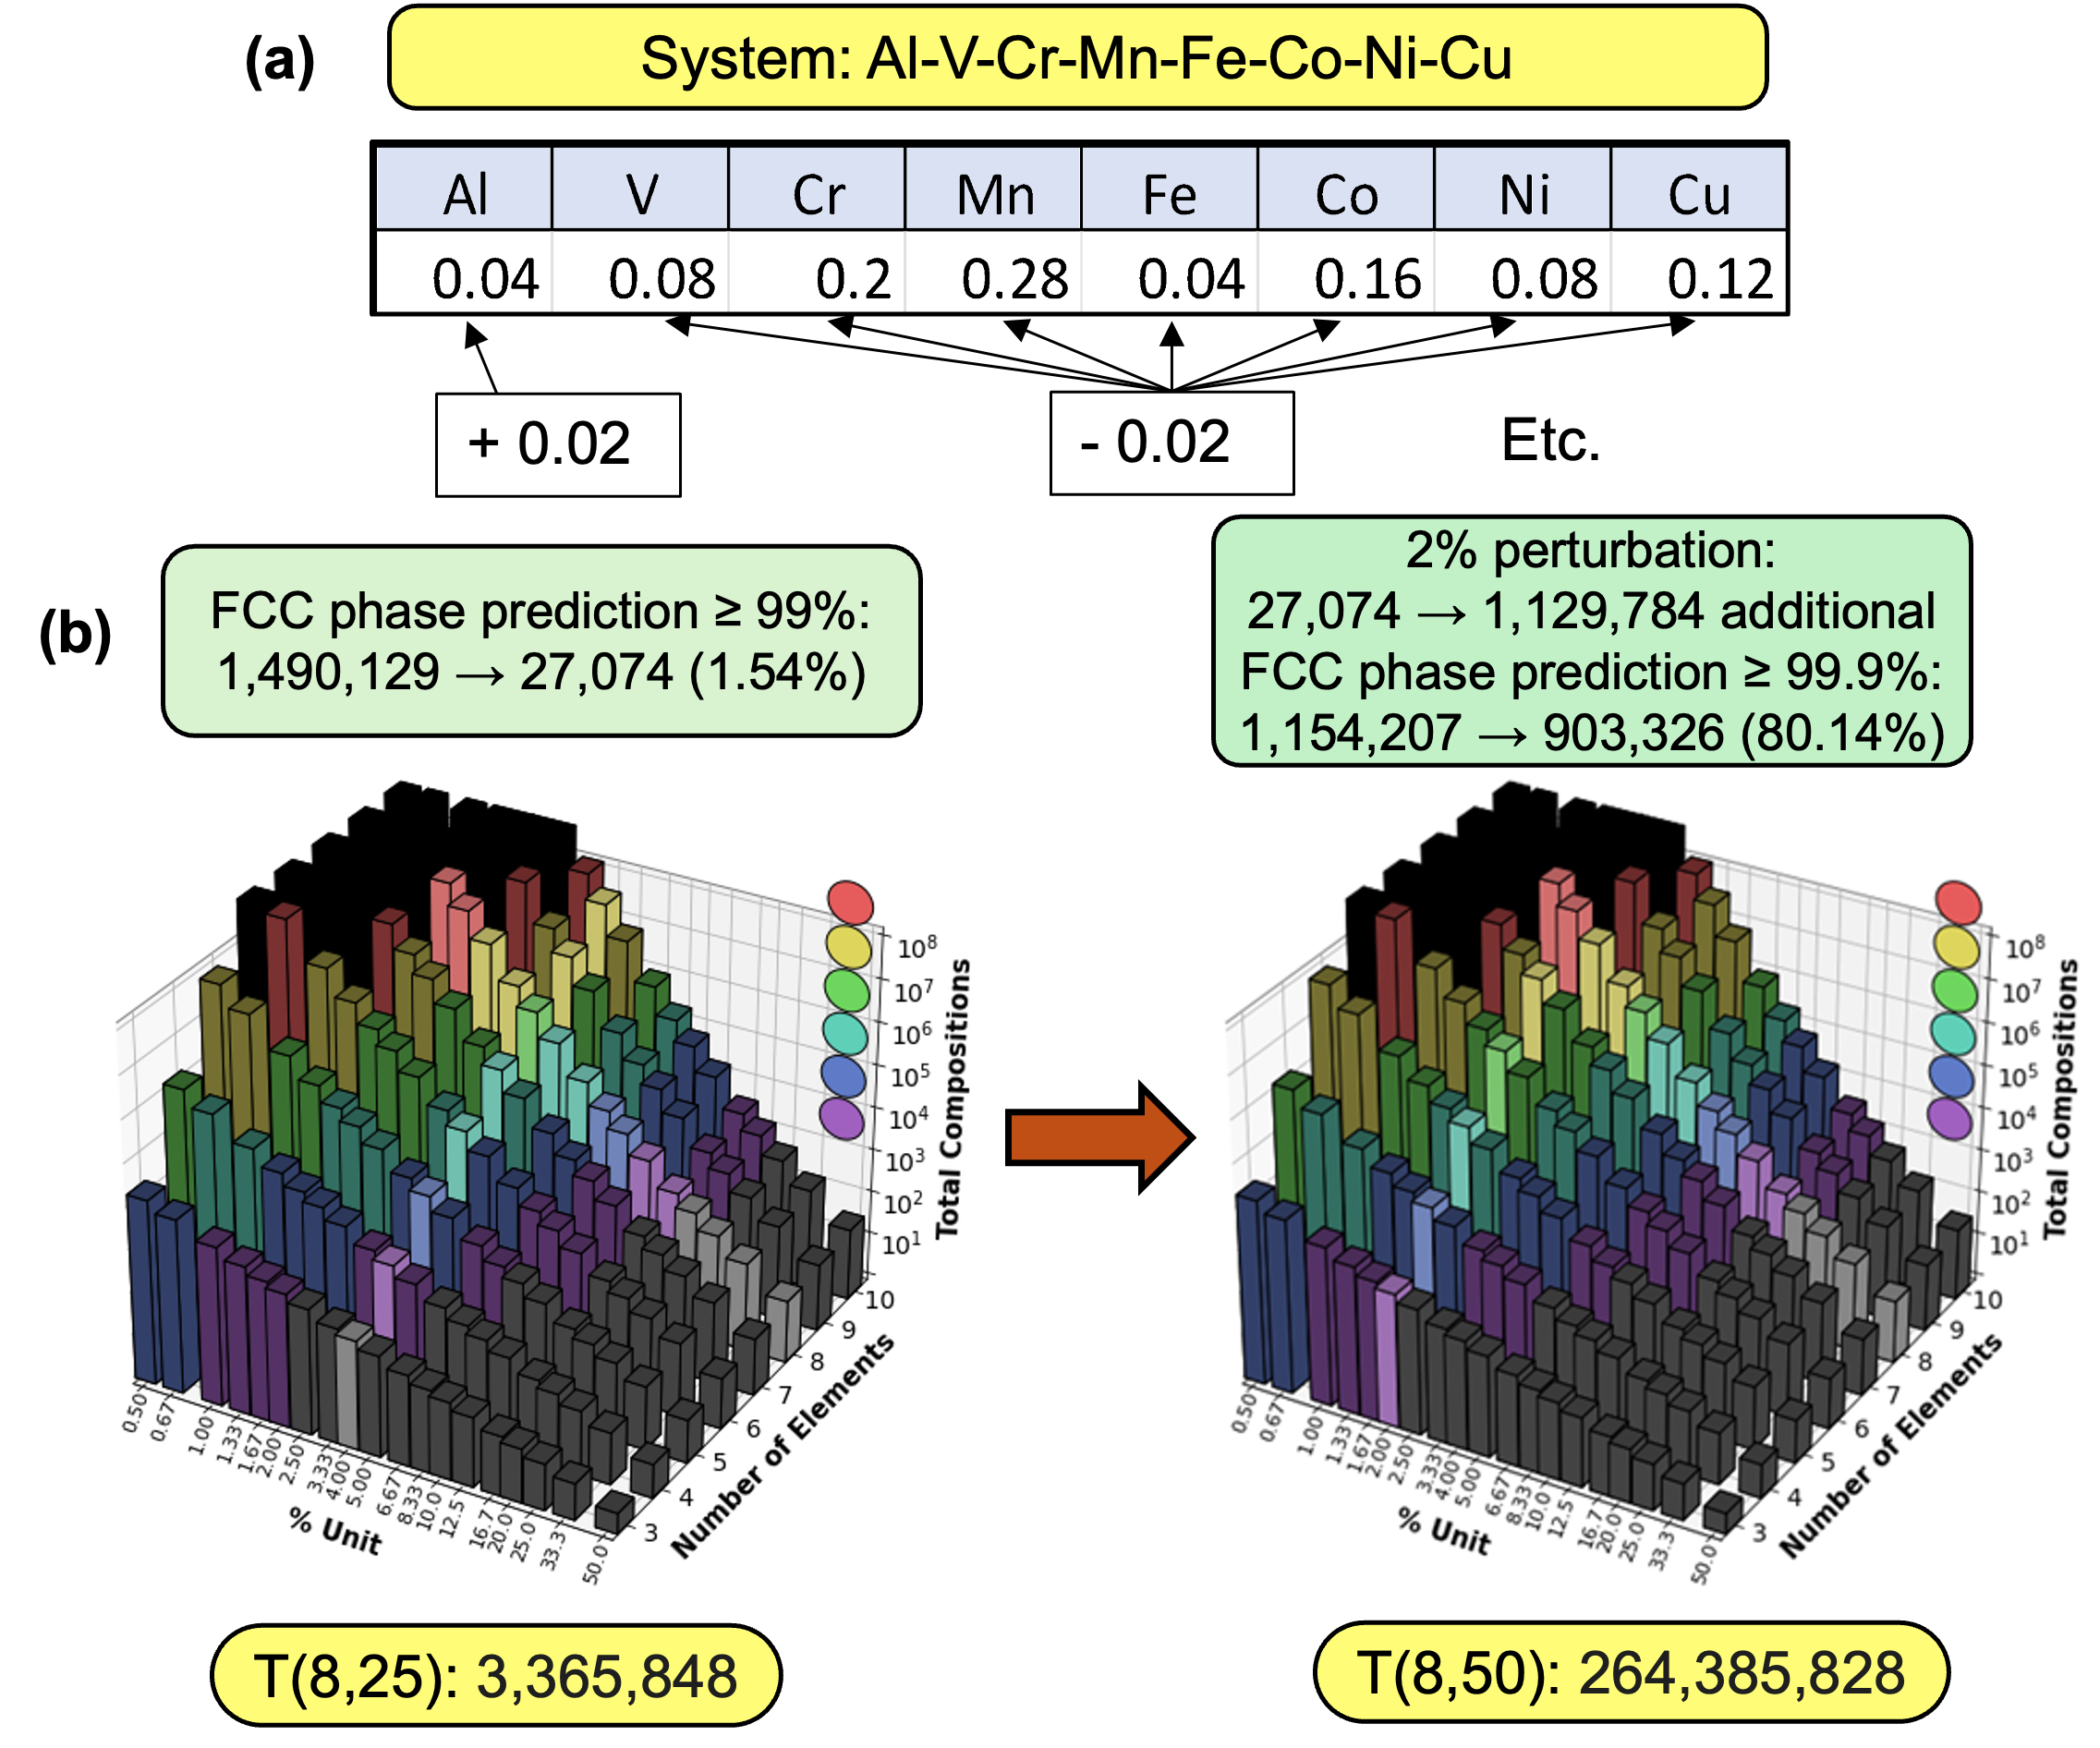
\includegraphics[width=0.7\linewidth]{Figures/perturbation_analysis_v2.png}
    \caption{Local FCC stability perturbation analysis. (a) Illustration of $\pm$2\,at.\% perturbations in 8D composition space. (b) Distribution of phase-stability outcomes: 80.1\% of perturbed alloys remain fully FCC (FCC $\geq 0.99$), while the remainder exhibit secondary phases such as BCC or SIGMA.}
    \label{fig:perturbation_analysis}
\end{figure}

By integrating this probability-aware feasibility modeling with our batch-mode EHVI acquisition, the current study robustly explores the complex high-entropy alloy design space. The framework prioritizes high-performance candidates while accounting for phase-stability uncertainties, ensuring adaptability to both model errors and experimental variability. This probabilistic strategy enhances the efficiency and reliability of the closed-loop materials discovery pipeline, accelerating the identification of novel, single-phase FCC alloys.


\subsubsection{Multi-Objective Optimization}

A multi-objective optimization problem is defined as
\begin{equation}
\label{eq:problem}
    \mbox{minimize}\,\,\,  \{f_1(\textbf{x}), ...,f_n(\textbf{x})\}, \textbf{x} \in \mathcal{X}
\end{equation}
where $f_1(\textbf{x}),\ldots, f_n(\textbf{x})$ are the objectives and $\mathcal{X}$ is the feasible design space. Typically, there is no single solution that simultaneously optimizes all objectives, rather, the solution is a set of non-dominated designs with trade-offs, which form the Pareto front in the objective space. In this context, the optimal solutions, $\mathbf{y}$, to a multi-objective optimization problem with $n$ objectives, are denoted as $\mathbf{y}\prec \mathbf{y'}$ and is expressed as
\begin{equation}
\begin{aligned}
   \{\mathbf{y}: \mathbf{y} & = (y_1, y_2, \ldots, y_n), \; y_i \leq y_i' \;\; \forall \; i \in \{1, 2, \ldots, n\}, &  \exists \; j \in \{1, 2, \ldots, n\} : y_j < y'_j\}
\end{aligned}{}
\end{equation} 
where $\mathbf{y}' = (y_1', y_2', \ldots, y_n')$ denotes any possible objective output.  
The set of $\mathbf{y} \in \mathcal{Y}$, where $\mathcal{Y}$ is the objective space, is known as the Pareto front.

There are several approaches to approximate/discover the Pareto front of a multi-objective optimization problem, such as the weighted sum approach~\cite{marler2010weighted}, the adaptive weighted sum approach~\cite{kim2005adaptive}, normal boundary intersection methods~\cite{das1998normal} and hypervolume indicator methods~\cite{beume2009s,bradstreet2010fast,emmerich2011hypervolume,fonseca2006improved,russo2013quick,yang2007novel,zitzler1999multiobjective}. In Bayesian optimization frameworks, hypervolume indicator techniques are well-suited to handle the probabilistic nature of Bayesian design and to approximate the Pareto front of solutions efficiently. Hypervolume refers to the space bounded by a fixed reference point and approximated Pareto front in the objective space. Thus, a hypervolume-based optimization is equivalent to maximizing the bounded space and pushing the approximation closer to the optimal Pareto front. The utility value function that drives the decision-making in multi-objective Bayesian optimization is 'Expected HyperVolume Improvement' (EHVI) which can be considered a multi-dimensional version of EI. 
We follow Ref.~\cite{zhao2018fast} where a recursive approach is suggested for the exact computations of hypervolume and EHVI for objective spaces of any dimensions. Simply put, the calculations are done by first decomposing the space bounded by reference point and Pareto front approximations into hyper-rectangles, and the overlapping parts are eliminated to obtain the exact hypervolume and expected hypervolume improvements.
The formula for calculating EHVI as outlined in~\cite{feliot2017bayesian} is given as
\begin{equation}
    \mathbb{E}[\textrm{{HVI}}({\mathbf{y}})] =\int_U \mathbb{P}(\mathbf{y} \prec{\mathbf{y}'})d{{\mathbf{y}'}}
    \label{Expected}
\end{equation}
where $\mathbb{P}(\mathbf{y} \prec \mathbf{y}')$ is the probability that $\mathbf{y}'$ dominates $\mathbf{y}$ and $U$ is the dominated hypervolume.
Given that we have an independent GP for each objective function, the posterior predictive of each GP given the data is a random variable identified as $y_i \sim \mathcal{N}(\mu_i , \sigma_i^2)$ where $ i\leq m  $ and $\mu_i,\sigma_i^2$ are the mean and variance of the $i^{th}$ objective accordingly. For a new potential solution in the design space, we have the following equation:
\begin{equation}
    \mathbb{P}(\mathbf{y} \prec \mathbf{y}') = \prod_{i=1}^m \Phi \left ( \frac{y_i' - \mu_i}{\sigma_i} \right )
    \label{prob}
\end{equation}
where $\Phi$ is the cumulative distribution function (CDF) of the standard normal random variable. Details regarding the closed-form expression of Eq.~(\ref{Expected}) can be found in Refs.~\cite{zhao2018fast,feliot2017bayesian,while2011fast,jaszkiewicz2018improved,khatamsaz2020efficient}.

\subsubsection{Multi-Source Modeling}


Often, there exist multiple computational models that estimate the same target property, however, each model is created based on different mathematical relations and simplifying assumptions. Consequently, some uncertainty is associated with their estimations and their level of fidelity differs. However, each model can provide valuable information about the target property such as variation trends and the existence of local minimums and maximums over the design space. Each model is considered a useful source of information and via combining information from these sources through a process known as model fusion, more accurate and less biased models can be created. Several approaches exist for fusing multiple sources of information, such as Bayesian modeling averaging~\cite{Clyde2003,Clyde2004,Draper1995,Hoeting1999,Leamer_1978,Madigan1994}, the use of adjustment factors~\cite{Mosleh1986,Reinert_2006,Riley2011,Zio_1996}, covariance intersection methods~\cite{Julier1997}, and fusion under known correlation~\cite{Geisser1965,Morris1977,Winkler_1981}. 
As more sources are incorporated into the fusion process, it is commonly expected to see a reduction in the variance of the quantity of interest estimates. However, this is not always the case with other fusion techniques such as Bayesian model averaging~\cite{Clyde2003,Clyde2004,Draper1995,Hoeting1999,Leamer_1978,Madigan1994,talapatra2018autonomous}, the use of adjustment factors~\cite{Mosleh1986,Reinert_2006,Riley2011,Zio_1996}, covariance intersection methods~\cite{Julier1997},
with the exception of fusion under known correlation ~\cite{Geisser1965,Morris1977,Winkler_1981}. 

Since we do not want to make any assumption on the hierarchy of information sources, it is crucial to establish the correlation between information sources before the fusion process. To do so, we use the reification technique to estimate the correlation coefficients between the different information sources~\cite{allaire2012fusing,thomison2017model}. Following the methodology outlined in previous studies such as Refs.\cite{allaire2012fusing,ghoreishi2018multi,ghoreishi2019JAIS,thomison2017model}, once the correlation coefficients are determined, the fused mean and variance at a specific design point \textbf{x} can be calculated using the method proposed in\cite{Winkler_1981}.

Following Ref.~\cite{Winkler_1981}, the fused mean and fused variance estimates from multiple predictions in the forms of normal distributions are defined as
\begin{equation}
\label{e:WinklerMeanGen}
\mathbb{E} [\hat{f}(\mathbf{x})]=\frac{\mathbf{e}^\textrm{T} \tilde{\Sigma}(\mathbf{x})^{-1}  \boldsymbol{\mu}(\mathbf{x})}{\mathbf{e}^\textrm{T} \tilde{\Sigma}(\mathbf{x})^{-1} \mathbf{e}}
\end{equation}
\begin{equation}
\label{e:WinklerVarianceGen}
\textrm{Var}\left(\hat{f}(\mathbf{x})\right) = \frac{1}{\mathbf{e}^\textrm{T} \tilde{\Sigma}(\mathbf{x})^{-1} \mathbf{e}}
\end{equation} 
where $\mathbf{e} = [1,\ldots,1]^\textrm{T}$, $\boldsymbol{\mu}(\mathbf{x}) = [\mu_1(\mathbf{x}),\ldots,\mu_m(\mathbf{x})]^\textrm{T}$ given $m$ information sources estimating the objective value at input location \textbf{x}, and $\tilde{\Sigma}(\mathbf{x})$ is the covariance matrix between information sources. Indicating rows and columns of the covariance matrix as $i$ and $j$ respectively, the diagonal elements are $\sigma_i^2$ and off-diagonal elements are $\bar{\rho}_{ij} \sigma_i \sigma_j$ where $\bar{\rho}_{i,j}$ is the correlation coefficient between information sources $i$ and $j$ at \textbf{x}. This correlation is calculated using a reification process based on the errors of two information sources $i$ and $j$ as:
\begin{equation}
\bar{\rho}_{ij}(\mathbf{x}) = \frac{\sigma_j^2(\mathbf{x})}{\sigma_i^2(\mathbf{x}) + \sigma_j^2(\mathbf{x})} \rho_{ij}(\mathbf{x}) + \frac{\sigma_i^2(\mathbf{x})}{\sigma_i^2(\mathbf{x})+\sigma_j^2(\mathbf{x})} \rho_{ji}(\mathbf{x}).
\label{e:VWrho}
\end{equation}
where $\rho_{ij}$ and $\rho_{ji}$ are:
\begin{equation}
\rho_{ij}(\mathbf{x}) = \frac{\sigma_i(\mathbf{x})}{\sqrt{\left(\mu_i(\mathbf{x})-\mu_j(\mathbf{x})\right)^2 + \sigma_i^2(\mathbf{x})}}.
\label{e:rho1}
\end{equation}

\begin{equation}
\rho_{ji}(\mathbf{x}) = \frac{\sigma_j(\mathbf{x})}{\sqrt{\left(\mu_i(\mathbf{x})-\mu_j(\mathbf{x})\right)^2 + \sigma_j^2(\mathbf{x})}}.
\label{e:rho2}
\end{equation}

The fused model, also a Gaussian process, is then created using fused means and fused variances as:
\begin{equation}
    \hat {f}^{\textrm{~fused}} (\textbf{x}) \sim \mathcal{N}(\mu^{\textrm{fused}}(\textbf{x}),\Sigma^{\textrm{fused}}(\textbf{x})).
\end{equation}

\subsubsection{Batch Bayesian Optimization}


A GP inference about the underlying objective functions largely depends on the point-wise correlation between data points that are computed using its kernel function. The length-scales are primary hyper-parameters of the kernel function that determine the strength of correlations in each direction of the input space, thus, setting optimal length-scales is crucial to accurately model the underlying objective function. There are systematic approaches to tune length-scales such as the maximum likelihood method \cite{Rasmussen:2005:GPM:1162254} and cross-validation. 
However, a potential problem here is that, most often, Bayesian optimization frameworks deal with expensive to evaluate, black-box objective functions with minimal data ~\cite{joy2020batch}. Therefore, in sparse high-dimensional input spaces, such a systematic approach is stuck in local optimums, not providing the optimal values to construct the GPs~\cite{couperthwaite2020materials}.

To tackle length-scale tuning issues, we use batch Bayesian optimization which the idea is to build a large number of GPs with randomly generated length-scales. This allows us to make different smoothness assumptions and reduce model mismatch risks caused by setting improper length-scales~\cite{joy2020batch}. Each GP makes a different inference about the underlying objective function given data, so the decision on the best next design to query will be different:
\begin{equation}
    \textbf{x}_{1:n} = \arg\max_{\mathbf{x} \in \chi}  \textrm{EHVI}^{N}(\textbf{x} | \textrm{GP}(\mathbb{D}_N,\theta_{1:n}))
\end{equation}
where there are $n$ different Gaussian processes built with different set of hyperparameters, $\theta$, given data $\mathbb{D}$. Depending on how many parallel experiments are allowed, also known as batch size, a k-medoid clustering problem is solved to select the proper number of candidates from all $n$ suggestions to query next. By solving the k-medoid problem, clusters of data points are formed by choosing cluster medoids such that it minimizes the distance between data points and the medoids.

\subsubsection{Constraint-aware EHVI}

To start the Bayesian optimization process, the first step is to filter the design space according to the imposed constraints. In this study, we are interested in fully FCC alloys and any alloys consisting of any different phases should be filtered. A preliminary step here is to check phase profiles of the entire search space using ThermoCalc. However, predictions from any computational model have some inaccuracies inherent to them, and design points closer to the constraint boundaries are more prone to such inaccuracies. As we get closer to the boundaries, the probability of getting a false prediction increases, and considering that many optimal designs are usually located close to boundaries, an absolute filtering approach may result in discarding many good designs.

Here, we propose to use a constraint-aware utility value function that considers the feasibility probability of design candidates in the calculations. Therefore, even if a candidate is predicted to be infeasible, it still can be included in the design space but with a lower probability of being feasible. thus, such candidates are given a second chance if they suggest significant improvements in terms of utility value. What we do here is to include falsely filtered designs in the BO search space using a probability that shows how confident we are in the feasibility of each candidate. Any candidate design that passes the filtering step is used to train a binary Gaussian process classifier (GPC). The good feature of a GPC is it provides uncertainty for its class membership predictions which is exactly what we are looking for here as the probability of belonging to the feasible class~\cite{Rasmussen:2005:GPM:1162254}. The filtered part of the design space is queried from the GPC and any candidate with the probability of being feasible larger than 80\% will be given a second chance to be included in the search space. However, the probability impacts the EHVI associated with those candidates:
\begin{equation}
    \textrm{EHVI(\textbf{x})}_{\textrm{constraint-aware}} = \textrm{EHVI}(\textbf{x})\times p_{\textrm{feasible}}(\textbf{x})
\end{equation}
Note that the initial candidates passing the filtering step are considered to be 100\% feasible and here we are trying to tackle false negative predictions to ensure we do not discard potentially good designs. The GPC will be updated as new experiments are run with new observations of feasible and infeasible training data.

\subsection{Data Management and Overall Workflow}

\subsubsection{Data Management}

Data management in prior BIRDSHOT study was organized around a \textbf{sample-centric framework}, designed to meet the distinct requirements of the VAM and DED synthesis workflows \cite{mulukutla2024illustrating}. This approach enabled end-to-end traceability from synthesis through characterization and analysis, supporting distributed collaboration and ensuring data integrity via natural version control. However, the path-dependent folder navigation imposed significant challenges for new users and complicated retrieval of specific results even for existing users. This experience highlighted the trade-off between strict data governance and user accessibility, motivating the adoption of a more discoverable, database-driven framework in subsequent studies.

In the current BIRDSHOT study, we implemented a \textbf{method-centric data architecture}, as shown in \autoref{fig:method_structure}, designed to maximize traceability, scalability, and efficiency while reducing redundancy. In this system, sample identifiers remain linked to synthesis origin, but folder organization treats design, processing and characterization methods as first-class entities beneath synthesis-level groupings. Sample folders use short, descriptive labels (e.g., \texttt{SEM}, \texttt{Tensile}, \texttt{NI}) to facilitate rapid identification, and measurement identifiers follow a hierarchical and extensible convention (\texttt{<SampleID>\_<Synthesis>\_<Technique>[\_<Subsample>][\_...]}). Metadata associated with each method, such as \texttt{sem-details.json} or \texttt{tensile-details.json}, is stored in structured JSON files within the corresponding method folders, allowing automated parsing, integration with downstream analysis pipelines, and programmatic traversal. For high-throughput synthesis, folders labeled by production batch capture shared processing metadata to minimize duplication while maintaining logical clarity and supporting future extensibility for new characterization techniques or processing steps. 


\begin{figure}[H]
    \centering
    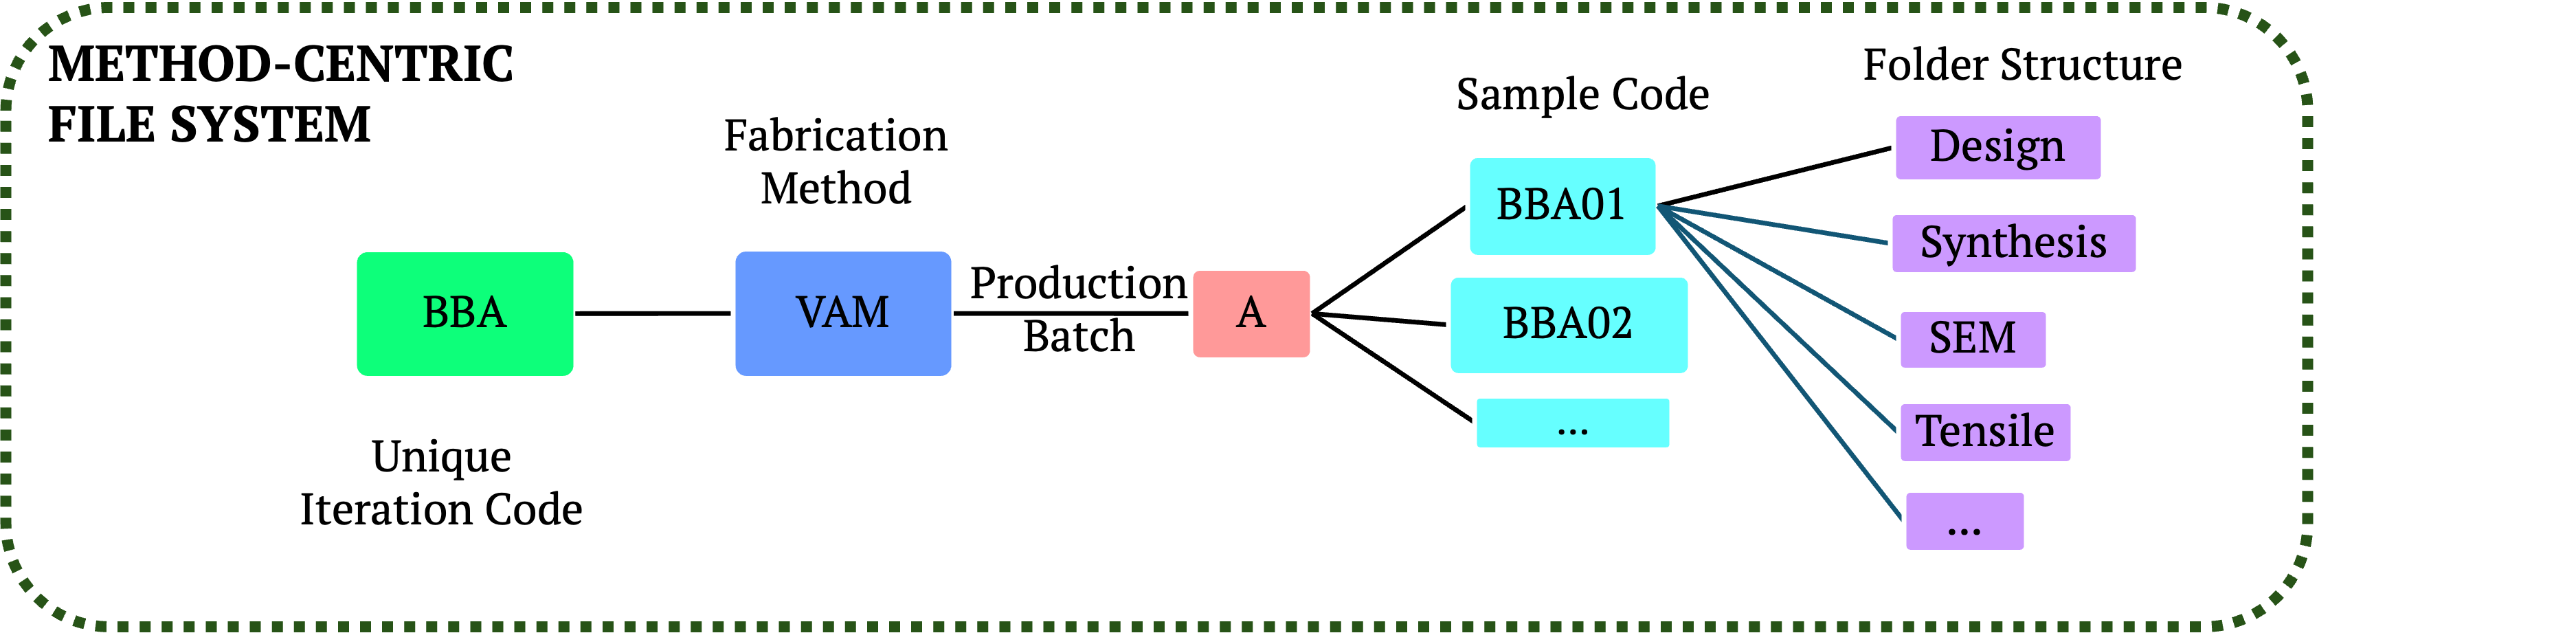
\includegraphics[width=0.9\linewidth]{Figures/file_structure.png}
    \caption{Folder structure illustrating synthesis-level grouping and method-focused organization.}
    \label{fig:method_structure}
\end{figure}

%check with Ali if the details below are accurate for IGSN

In addition, each candidate alloy in this study is assigned an International Generic Sample Number (IGSN), a globally unique, resolvable identifier for physical samples, thereby linking the physical specimens, their metadata, and downstream analytical results in a persistent, cross-platform framework. IGSNs are issued and managed under the IGSN–DataCite partnership, ensuring sustainability and interoperability across research data systems \cite{datacite-igsn-ids}. 

By design, IGSN identifiers behave like DOIs, they are registered in a dedicated IGSN catalog within the DataCite system and resolved using standard DOI infrastructure, but are distinguished semantically as “physical object” identifiers. The metadata for each IGSN follows the DataCite Metadata Schema, including mandatory fields such as identifier, creator, title, publisher, publication year, and resource Type, along with recommended fields like related identifier, contributors, dates, descriptions, and geolocation when applicable \cite{igsn-metadata-schema}. In particular, our sample hierarchy is reflected in the related Identifier fields so that parent–child relationships (like subsamples) are explicitly recorded in the IGSN metadata. Because IGSNs are globally registered and resolvable, they support FAIR principles, especially findability and interoperability, by enabling external users (or data infrastructures) to unambiguously reference and access sample information, even beyond our internal data ecosystem. All IGSNs, along with full citation metadata and mapping to our internal identifiers, are included in the \textbf{SI}, so that any researcher can trace back from published data to the original sample record.

\subsubsection{Integrated High-throughput Workflow}

The BIRDSHOT represents a highly integrated and complex materials discovery workflow, combining computational design, high-throughput synthesis, characterization, and simulation to optimize multiple mechanical properties simultaneously. To illustrate the complexity and sequential/iterative nature of the study, all major steps from candidate alloy suggestion, through synthesis and sample preparation, to experimental characterization and FEM-based simulations are presented in the flowchart shown in \autoref{fig:workflow}. This figure emphasizes the interdependent and multi-stage processes involved, highlighting the substantial technical and logistical complexity of the study. The figure provides a clear overview of the numerous interrelated operations required to identify optimal material compositions while ensuring traceable data management throughout the discovery process.

\begin{figure}[H]
    \centering
    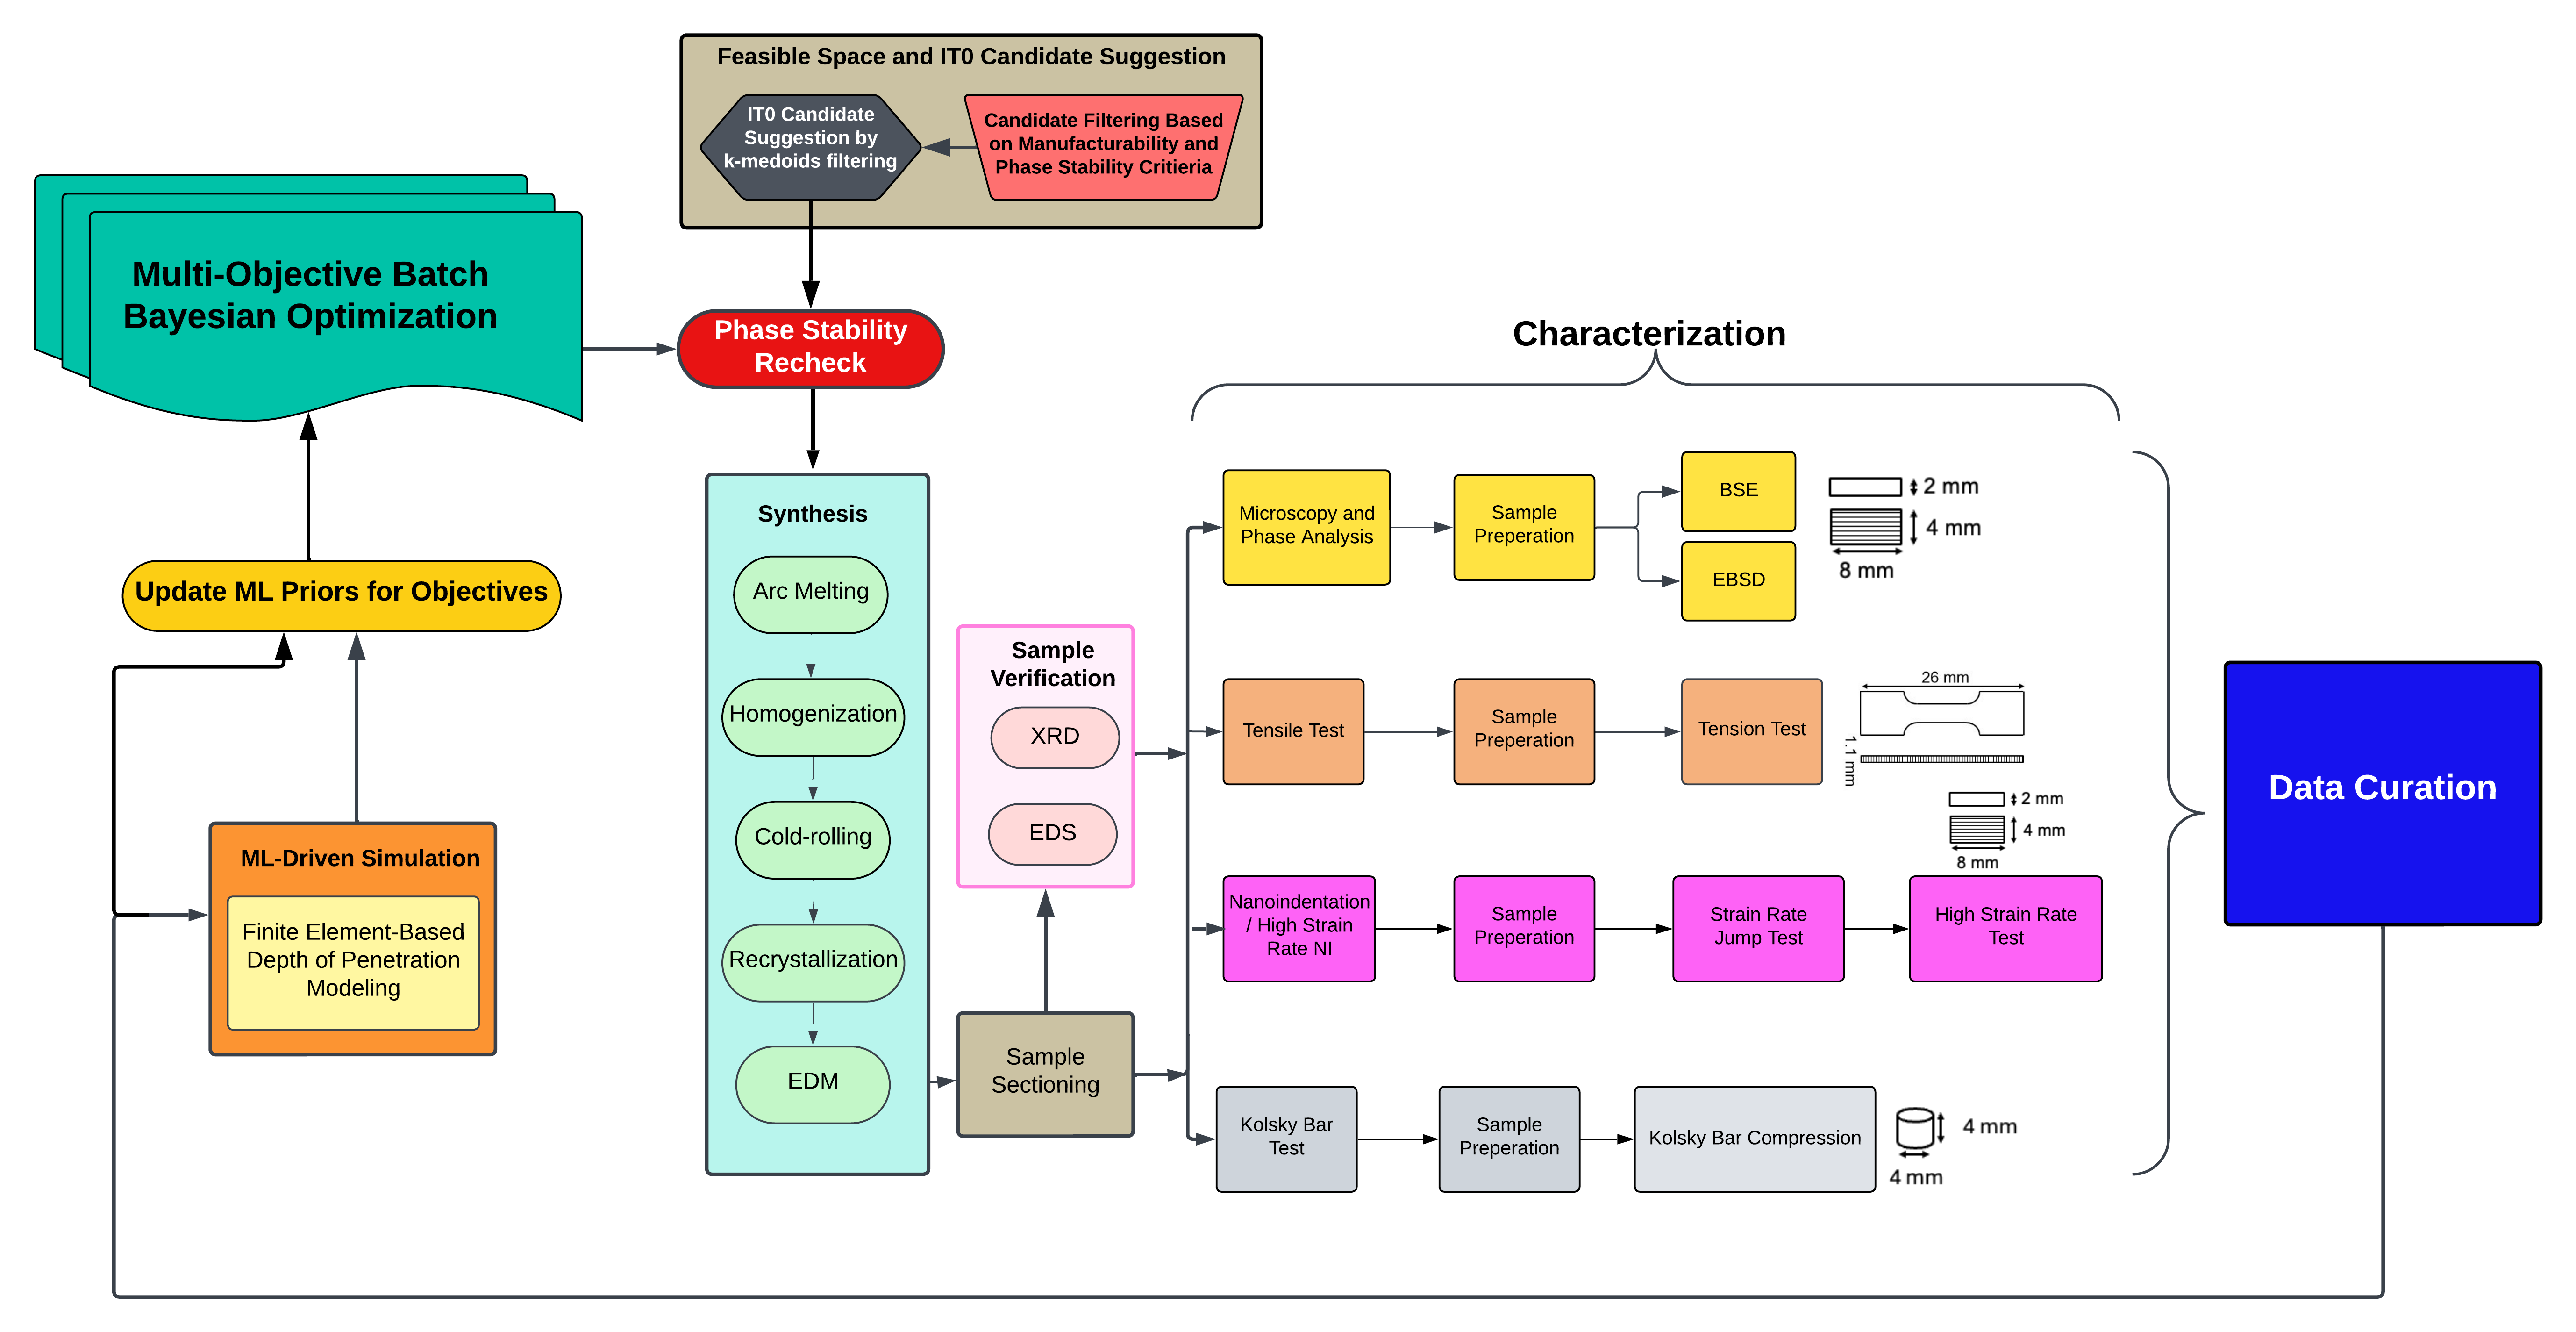
\includegraphics[width=0.95\linewidth]{Figures/BIRDSHOT Workflow.png}
    \caption{Comprehensive and Iterative BIRDSHOT workflow from candidate suggestion to synthesis, sample preparation, characterization, simulation and Bayesian Optimization for suggestion of next batch of candidates.}
    \label{fig:workflow}
\end{figure}


It integrated computational and experimental workflows to maximize key mechanical properties, including yield strength (YS), the UTS/YS ratio, strain at UTS, and the dynamic-to-quasi-static strength ratio (H$_\text{dyn}$/H$_\text{qs}$), while minimizing penetration depth. Overall, candidate alloy suggestion employed multi-objective optimization integrated with machine learning models and Bayesian frameworks, systematically reducing the design space from approximately 3.4 million potential compositions to roughly 27,000 feasible alloys based on predicted phase stability, manufacturability, and target mechanical performance. High-throughput synthesis was carried out using Vacuum Arc Melting (VAM), followed by extensive characterization including tensile testing, Nano-Indentation (NI), and Kolsky Bar experiments to evaluate mechanical behavior. Finite Element Modeling (FEM) was used in parallel to predict penetration depth under extreme loading, providing complementary insights to experimental measurements. Automation was critical throughout the study, enabling systematic data acquisition, processing, and workflow management. The method-centric organization and integrated workflow ensured that experimental data, computational predictions, and derived material properties were fully traceable, programmatically accessible, and reproducible, supporting rapid iteration and data-driven alloy optimization.

